\documentclass[a4paper,12pt]{scrreprt}

\usepackage[english]{babel}
\usepackage[utf8x]{inputenc}
\usepackage{ucs}

\usepackage{natbib}
\bibliographystyle{unsrtnat}

\usepackage{amssymb}

\usepackage{hyperref}

\usepackage{graphicx}
\usepackage{caption}
\usepackage{subcaption}
\usepackage{float}

\title{Kingdom of Kush - 0 A.D. Mod - Specification}

\begin{document}

\maketitle

\abstract{This is the development specification for the Kushite Mod. The Kushite Mod adds the Kushite civilization to the real time strategy game \href{https://play0ad.com/}{0 A.D.}.}

\tableofcontents

\chapter{Units, Buildings and Technology Tree}

Buildings:

\begin{itemize}
	\item Temple
	\item Civic Center
	\item Storehouse $\rightarrow$ TODO Research \& Sketch
	\item House \checkmark
	\item Blacksmith $\rightarrow$ TODO Sketch
	\item Field
	\item Farmstead
	\item Corral
	%\item (TODO Something like a Mill)
	\item Market $\rightarrow$ TODO Sketch
	\item Dock
	\item Barracks $\rightarrow$ TODO Research (how did they look like?)
	\item Fortress
	\item Sentry Tower (Wooden Tower)
	\item Defense Tower \checkmark
	\item Outpost $\rightarrow$ TODO Research (how did they look like?)
	\item Low Wall + Gate (Mostly wooden, but we could use a brick wall instead)
	\item City Wall + City Gate (Stone Wall)
	\item Wonder
	\item Special Structures
	\begin{itemize}
		\item Beja Embassy  
		
		\item Nubia Embassy $\rightarrow$ TODO Research (Do we need one?)
		\item Waterwheel [Saqiya (Sakia)] $\rightarrow$ TODO Do we need one? Farming Bonus?
	\end{itemize}
\end{itemize}

Units:

\begin{itemize}
	\item Woman worker $\rightarrow$ TODO Research (how did they look like? Avoid racial bias)
	\item Basic infantry/cavalry workers $\rightarrow$ TODO Research (how did they look like?)
	\item Priest
	\item Meroitic Spear Cavalry
	\item Nubian Horse Archer
	\item Chariots
	\item Beja Swordsman (mercenaries)
	\item Beja Spearman (mercenaries)
	\item Beja Camel Warrior (mercenaries)
	\item Siege Weapons
	\begin{itemize}
		\item Battering Ram
		\item Siege Tower
	\end{itemize}
	\item Naval Units
	\begin{itemize}
		\item Fishing Boat $\rightarrow$ TODO Research (papyrus or wooden?) \& Sketch
		\item Light Warship
		\item Medium Warship
	\end{itemize}
	\item Trader
	\begin{itemize}
		\item Trader (land)
		\item Trader (water)
	\end{itemize}
	\item Champion Units
	\begin{itemize}
		\item Nubian Bowmen
		\item TODO other elite units
	\end{itemize}
	\item Heros $\rightarrow$ TODO Research (Important Queens/Kings, Priests etc.)
	\begin{itemize}
		\item Arikhankharer TODO Research \& Decision
		\begin{itemize}
			\item With the ability to recruit 1 to 5 dogs which automatically guard him (like in AoE III) would be an interesting idea. Because of the dogs, any unit within his area of influence would get a defense bonus.  
		\end{itemize}
		\item Amanirenas ("Queen Candace" Strabo)
		\item Amanitore ("Candace, Queen of the Ethiopians" Bible)
	\end{itemize}
\end{itemize}

Special Technologies:

\begin{itemize}
	\item Iron production bonus
	\item Cattle bonus
\end{itemize}

Agriculture:

\begin{itemize}
	\item Wheat fields
	\item Corral
	\begin{itemize}
		\item Sanga Cattle
		\item Goat
		\item Sheep
	\end{itemize}
\end{itemize}
Special Features:

\begin{itemize}
	\item Nubian Bowmen shoots poisoned arrows
\end{itemize}

Fauna:

\begin{itemize}
	\item Date trees as food resource
\end{itemize}

\section{Buildings}

\subsection{Beja Embassy}

\paragraph{Phase:} Town or City?\\

The embassy could be a simple Kushite rectangular structure with two Beja tents next to it, and some round shields and lances lying around.\\

The Beja embassy can recruit Beja mercenaries.

\subsection{Blacksmith}

\paragraph{Phase:} Town\\

\begin{figure}[H]
	\centering
	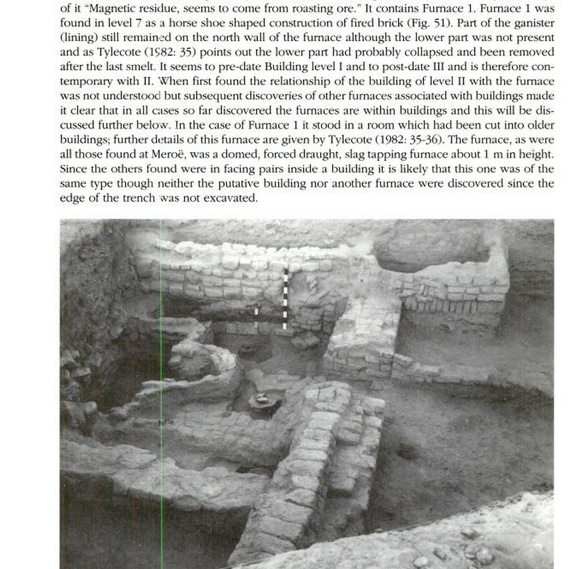
\includegraphics[width=\textwidth]{img/blacksmith/blacksmith_layout}
	\caption{This excerpt from "The capital of Kush" describes a furnace for iron-smelting. It was dome shaped, and located within a building, like all the furnaces in Meroe. Maybe the blacksmith for the Kushites could be a simple rectangular building in a courtyard with a small secondary building with a chimney and an orange glow coming from the doorway, to represent this smelting process.  }
\end{figure}

\subsection{Civic Center}

\paragraph{Phase:} Village\\

Of all the buildings, civic center should be based on the typical Kushite palaces, like the one at Karanog (see \ref{fig:karanog_governor_palace}). These palaces were administrative centers, storehouses for food and luxery products/trade items, and served as living quarters to governors. This is where dignitaries would be received, and policies would be made. Literally town centers! Maybe reduce the height from 3 stories to 2 stories. Some miniature obelisks or stone inscriptions decorating the front. A set of pillars with papyrus shaped capitols \ref{fig:papyrus_capitol} at the entrance, with a single stone slab on top, to make it look inviting. 

\begin{figure}[H]
	\centering
	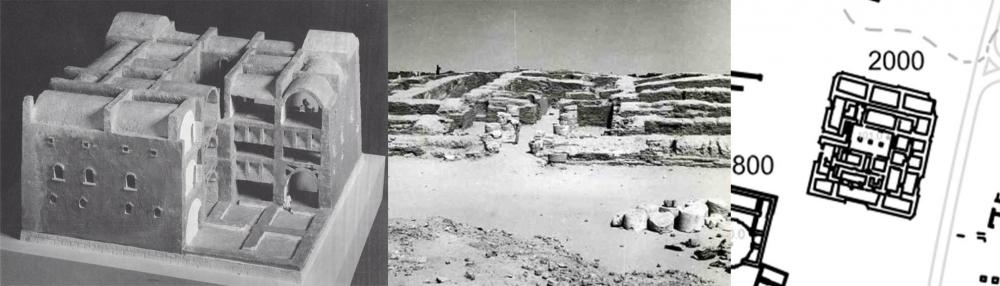
\includegraphics[width=\textwidth]{img/civic_center/three_palace_pictures}
	\caption{Meroitic governors' residence at Karanog (left), and palace at Wad Ben Naqa (center) and Naqa (right). These are literally town centers.}
\end{figure}

\begin{figure}[H]
	\centering
	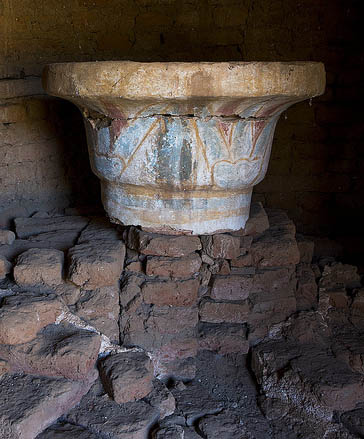
\includegraphics[width=\textwidth]{img/civic_center/papyrus_shaped_capitols}
	\caption{A well preserved example of a Meroitic papyrus capital from the Royal baths at Meroe, which would have topped a column (pillar). Would be nice for an entrance portico.}\label{fig:papyrus_capitol}
\end{figure}

\begin{figure}[H]
	\centering
	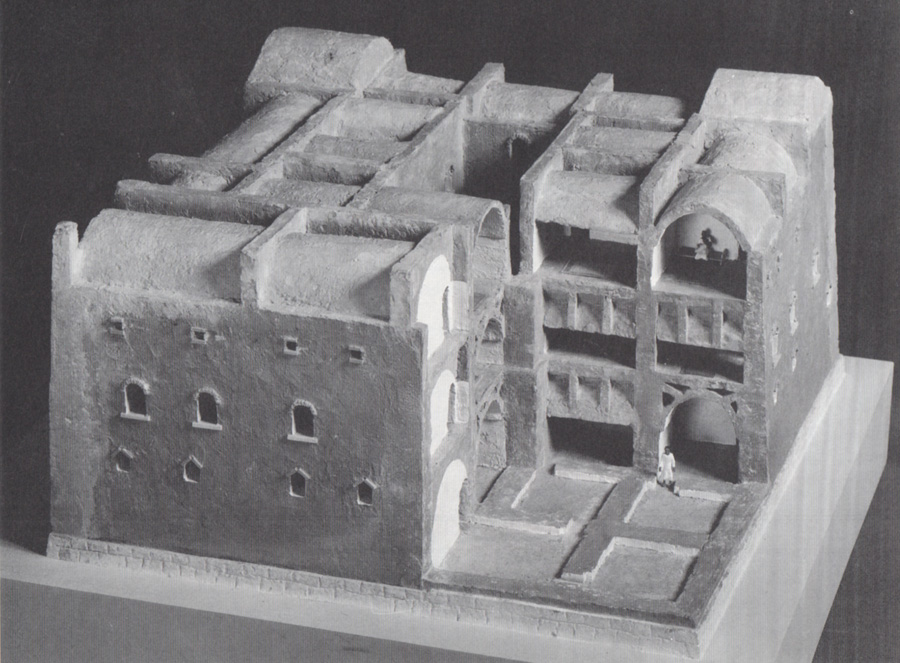
\includegraphics[width=\textwidth]{img/civic_center/governor_palace_karanog}
	\caption{A small governors' palace in Karanog, lower Nubia. This building features typical Nubian architecture, with vaulted ceilings, open courtyard and square design. Small windows and thick walls on the lower floor hint at a defensive purpose. A lavishly decorated 2nd floor served as the living space for the governor and his family "Fabricated by Christ Ray, in collaboration with David O'Connor and Stacey Olson, from plans an descriptions of the 1907 excavation"}\label{fig:karanog_governor_palace}
\end{figure}

\subsection{Corral}

\paragraph{Phase:} Village\\

It is possible to breed goats, sheep and Sanga cattle in the corral.

%TODO how should the corral look like?

\subsubsection{Goat}

0 A.D. has already a model for goats the Kushites Mod will reuse it.

\subsubsection{Sheep}

0 A.D. has already a model for sheep the Kushites Mod will reuse it.

\subsubsection{Sanga Cattle}

The specific species of cattle you're looking for is Sanga cattle, also known as "Bos Taurus Africanus". An indigenous, African-domesticated species. Many subspecies exist throughout the continent (of which Ankole Watusi is one example). Smaller, short-horned, modern day cattle of Northern Sudan have been mixed with Indian Zebu's over the past centuries. I think it goes without saying that cattle was extremely important to Kush.\\

\begin{figure}[H]
	\centering
	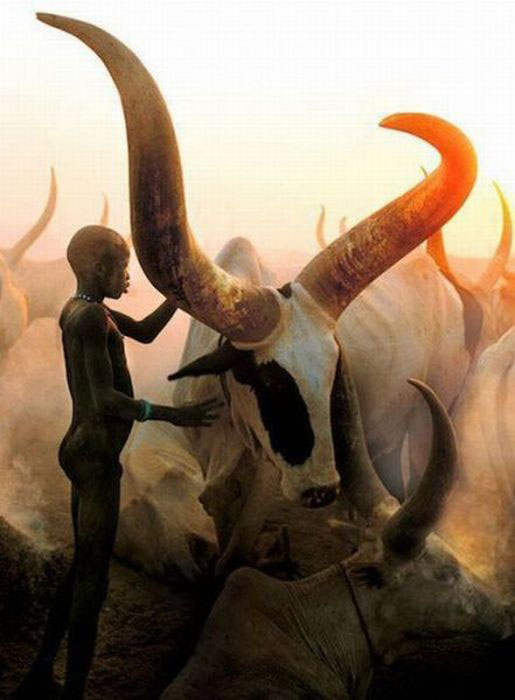
\includegraphics[width=\textwidth]{img/corral/sanga_cattle_dinka}
	\caption{Massive horned cattle of the Dinka, in modern day South-Sudan}
\end{figure}

The Sanga cattle can be breed in the corral. The cost will be something around 200-300 food and they provide in return 500 food. In addition the Kushites have can develop a breeding bonus technology, which lowers the breeding (training) time by 10\%. Another technology makes Sanga Cattle breeding less costly. By developing the breeding cost bonus, Sanga cattle will cost 50-100 less food.\\

\begin{figure}[H]
	\centering
	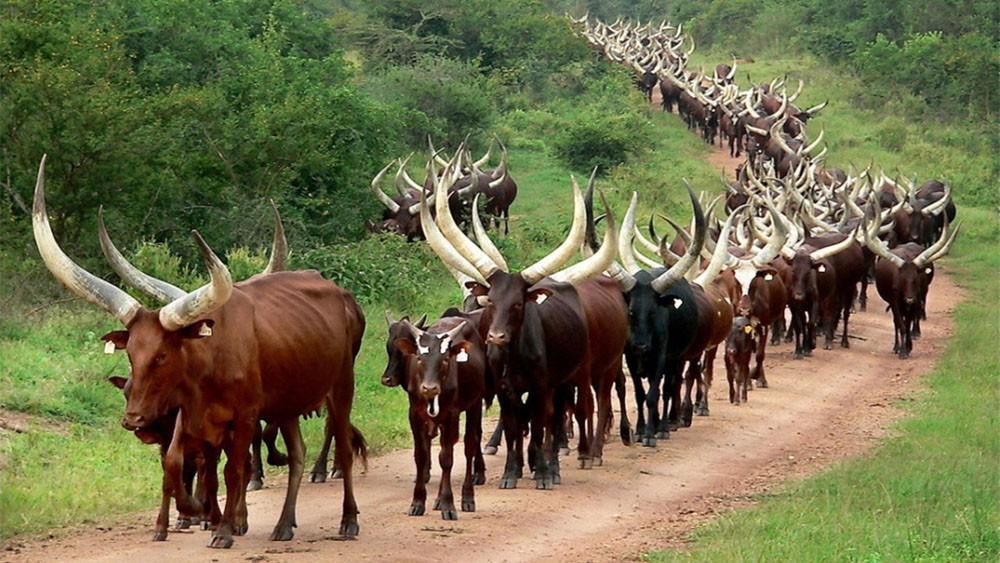
\includegraphics[width=\textwidth]{img/corral/herd_of_sanga_cattles}
	\caption{Massive horned cattle of the Dinka, in modern day South-Sudan}
\end{figure}

\begin{figure}[H]
	\centering
	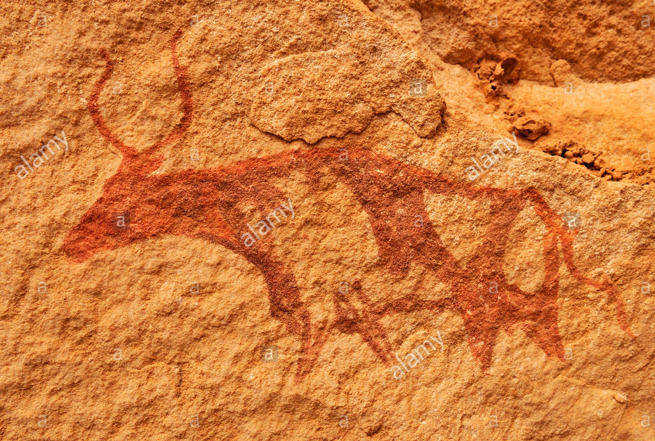
\includegraphics[width=\textwidth]{img/corral/neolethic_rock_art_sanga_cattle}
	\caption{Neolithic Rock Art, from Algeria. Similar scenes are widespread in the Sahara, before the aridification of the desert in modern times. This cow might have well been the ancestor to the cows pictured above.}
\end{figure}

\subsection{Defense Tower}

\paragraph{Status:} 3-D Model Created\\
\paragraph{Phase:} Town\\


\begin{figure}[H]
	\centering
	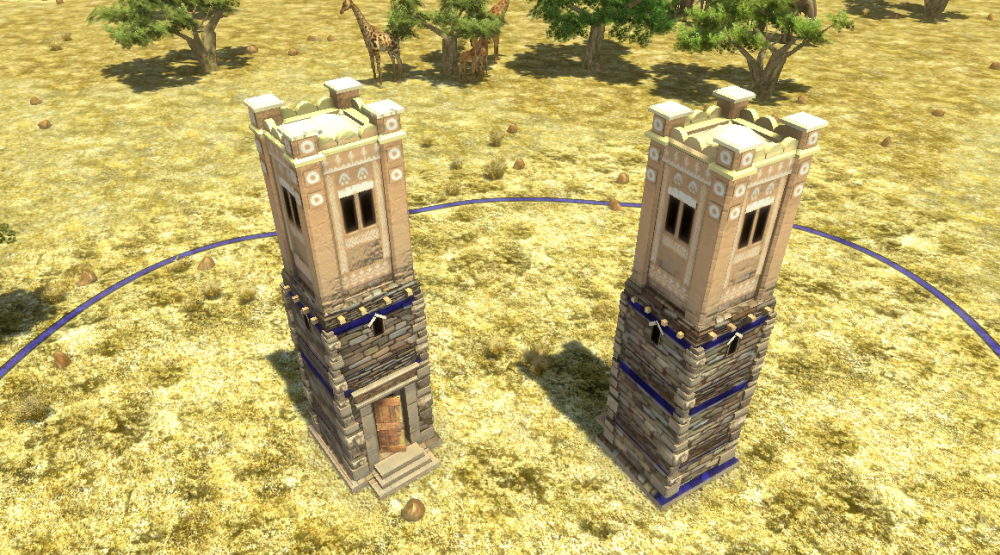
\includegraphics[width=\textwidth]{img/tower/tower}
	\caption{3-D model of tower by @LordGood}
\end{figure}

\subsection{Farmstead}

\paragraph{Phase:} Village\\

The model of a large Meroitic era, beehive structure at Wad Ben Naqa. Some claim it to be a granary (silo), and others a temple. At Gala Abu Ahmed, several similar, although seriously less monumental structures were excavated. The people of that excavation were pretty sure their structures were granaries. Grain would be added through a hole at the top with a tall ladder. It would subsequently be taken from an access hole at the bottom when needed. The silos at Abu Ahmed could have fed several hundred men for a year. Both the structures at Abu Ahmed and at Wad ben Naqa were plastered white on the outside. The structures are so architecturally unique. Their unique shape would be quite cool as a model for the farm building.

\begin{figure}[H]
	\centering
	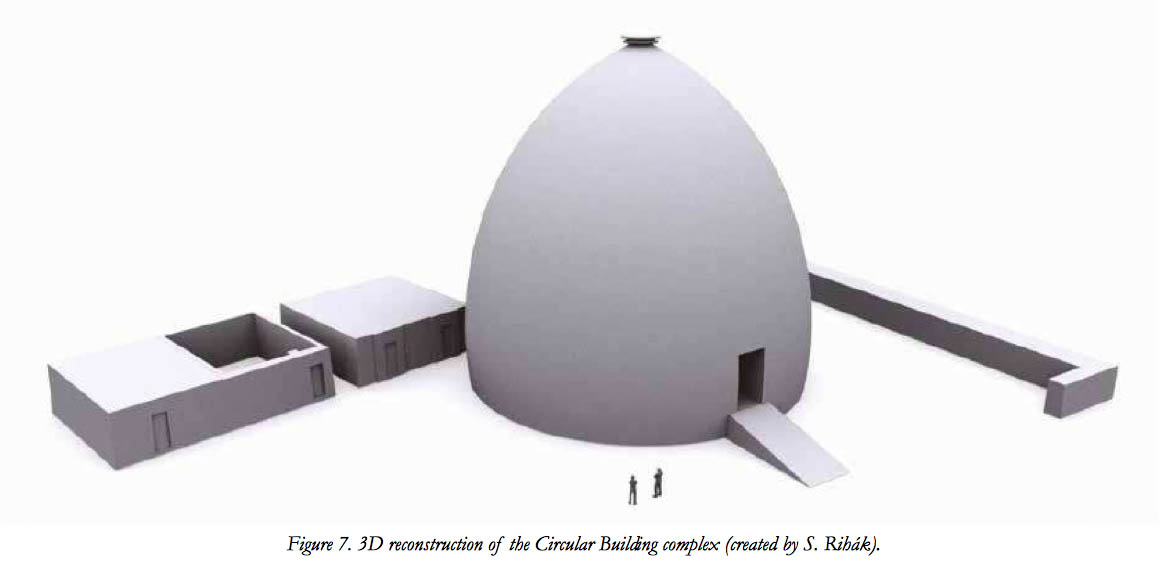
\includegraphics[width=\textwidth]{img/farmstead/3d_reconstruction}
	\caption{3d reconstruction of the Circular Building (WBN 50) at Wad Ben Naqa. Some claim it is a silo. Others say that with a diameter of 18meters and a height of 20 meters, it was too monumental to be a silo. An access ramp hints at its possible use as a shrine or temple. Access ramps are common in religious structures. }
\end{figure}

\begin{figure}[H]
	\centering
	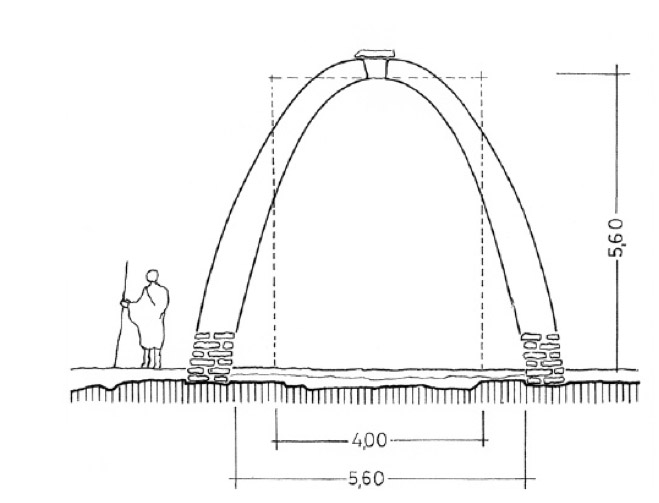
\includegraphics[width=\textwidth]{img/farmstead/sketch_granaries_gala_abu_ahmed}
	\caption{A model of one of the granaries at Gala Abu Ahmed. Sand stone foundation, and brick for its upper courses. Plastered with white lime plaster.}
\end{figure}

\begin{figure}[H]
	\centering
	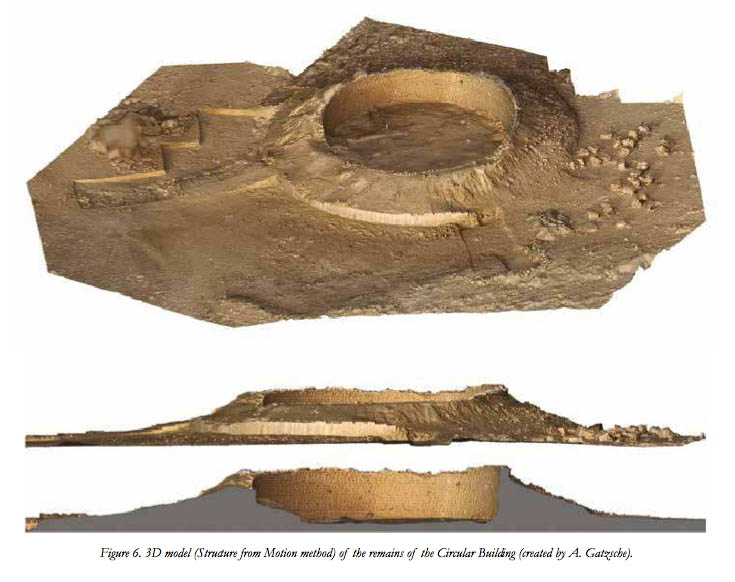
\includegraphics[width=\textwidth]{img/farmstead/3d_reconstruction_circular_building}
	\caption{3d image of the remains of the "circular building" (WBN 50) at Wad Ben Naqa.}
\end{figure}

\subsection{Field}

\paragraph{Phase:} Village\\

\paragraph{Short answer:} Reuse the field from the main Game.

\paragraph{Explanation:}

Their fields shouldn’t necessarily look different from any other field in the game. They grew barley, wheat, millet, sorghum and cotton.

\subsection{Fortress}

The site called “Gala Abu Ahmed”. Don’t get stuck up on the name though, radiocarbon dating puts this place between 700BCE – 350BCE, which makes it, Napatan and early Meroitic. It’s quite a large, trapezoid fort, with thick dry-stone walls, bastions, and staircases to reach the upper walls and bastions. Sadly, as with many places in Sudan, the site was mined for building materials for the nearby, modern town, making it difficult to estimate its height in the old days, but some walls still reach 4 meters. Notable feature, as with all Meroitic fortifications, is the conspicuously small gate entrance, undoubtedly a security measure making access more difficult. 

%TODO Type in text about history research

\begin{figure}[H]
	\centering
	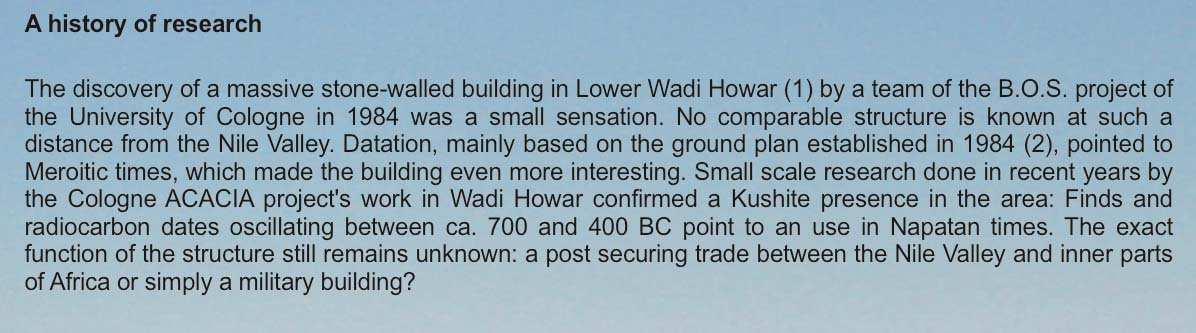
\includegraphics[width=\textwidth]{img/fortress/history_of_research}
	\caption{Aerial view of the main entrance gate to Gala Abu Ahmed. A very narrow passage way, with a pair of stairs in the middle, leading up to the walls and bastions.}
\end{figure}

\begin{figure}[H]
	\centering
	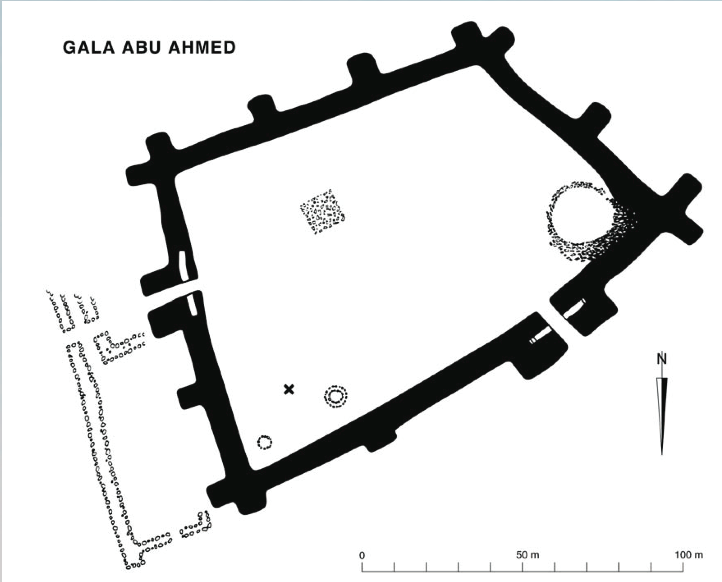
\includegraphics[width=\textwidth]{img/fortress/gala_abu_ahmed}
	\caption{Plan of Gala Abu Ahmed}
\end{figure}

\begin{figure}[H]
	\centering
	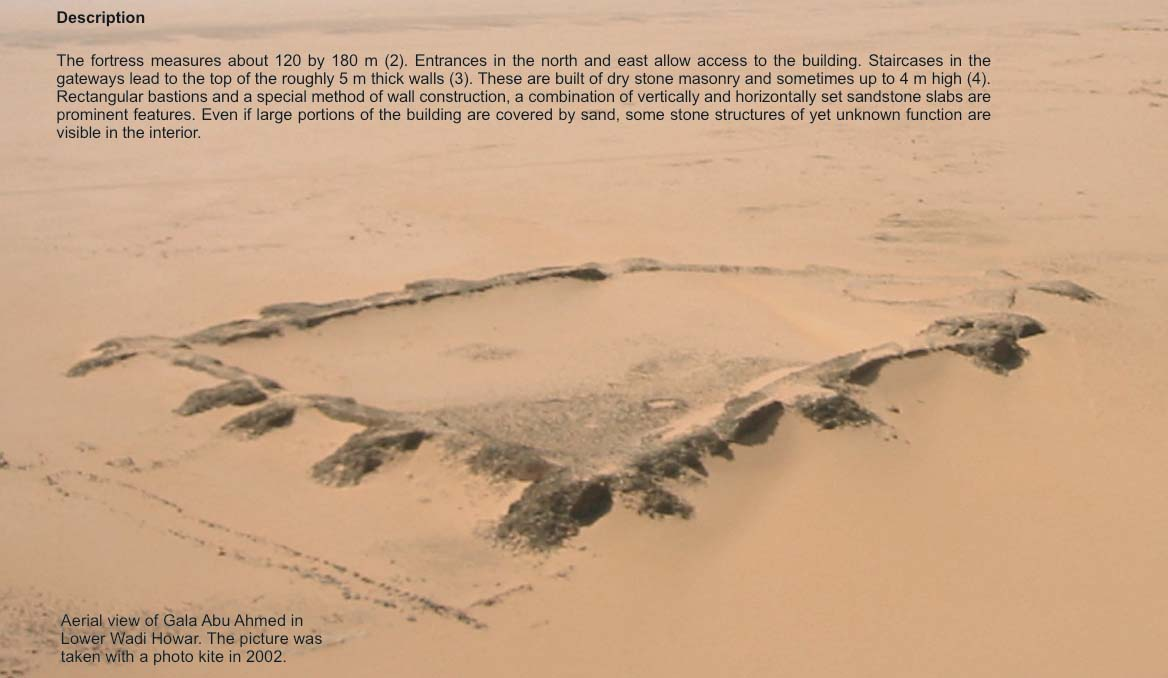
\includegraphics[width=\textwidth]{img/fortress/aerial_view_gala_abu_ahmed}
	\caption{Aerial view of Gala Abu Ahmed}
\end{figure}

\begin{figure}[H]
	\centering
	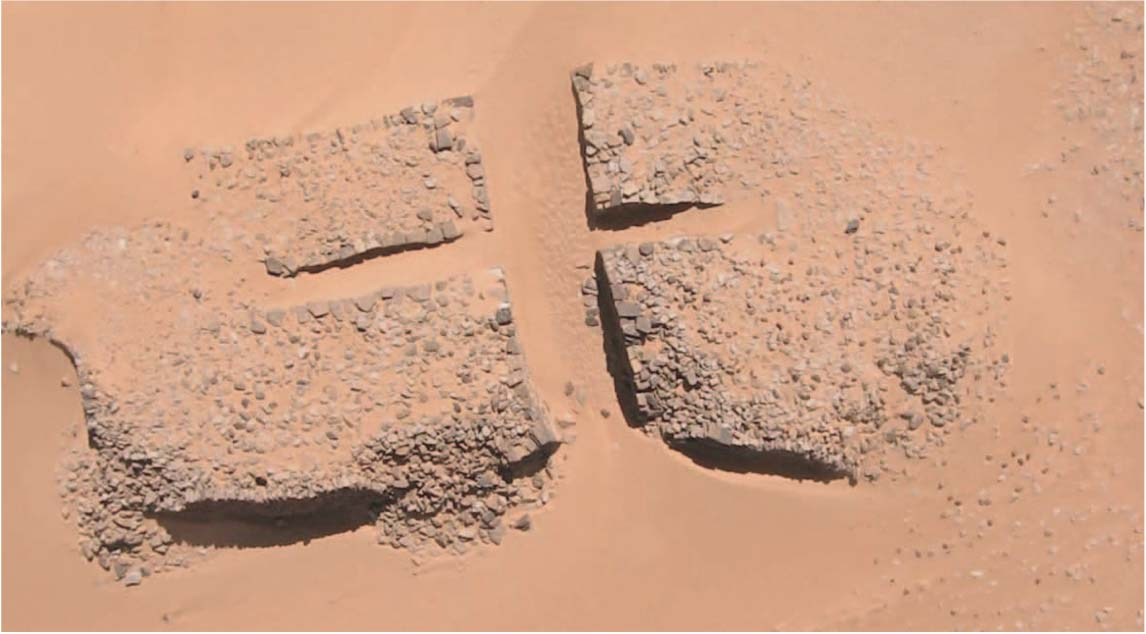
\includegraphics[width=\textwidth]{img/fortress/aerial_view_entrance_bastion}
	\caption{Aerial view of the main entrance gate to Gala Abu Ahmed. A very narrow passage way, with a pair of stairs in the middle, leading up to the walls and bastions}
\end{figure}

\begin{figure}[H]
	\centering
	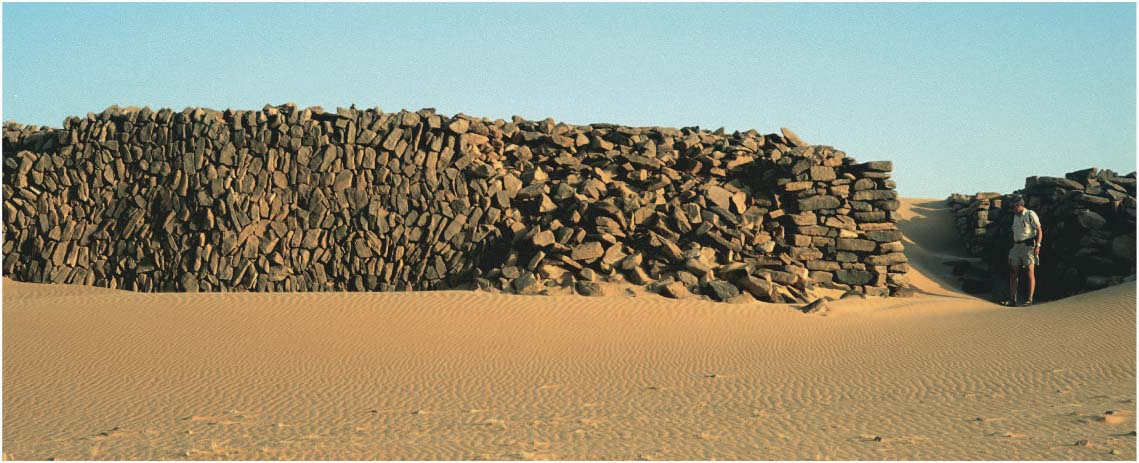
\includegraphics[width=\textwidth]{img/fortress/dry_stone_wall_gala_abu_ahmed}
	\caption{Beautiful example of Kushite dry-stone walls in Gala Abu Ahmed}
\end{figure}

A final note on fortifications. The massive Middle Kingdom fortresses, such as Semna and Buhen, regularly fell to Kushite hands from the 2nd intermediate period onwards, well into Ptolemaic times. Although originally built by Egyptians, their style may well have influenced later Meroitic fortifications, and can be used for stylistic hints in models.

\begin{figure}[H]
	\centering
	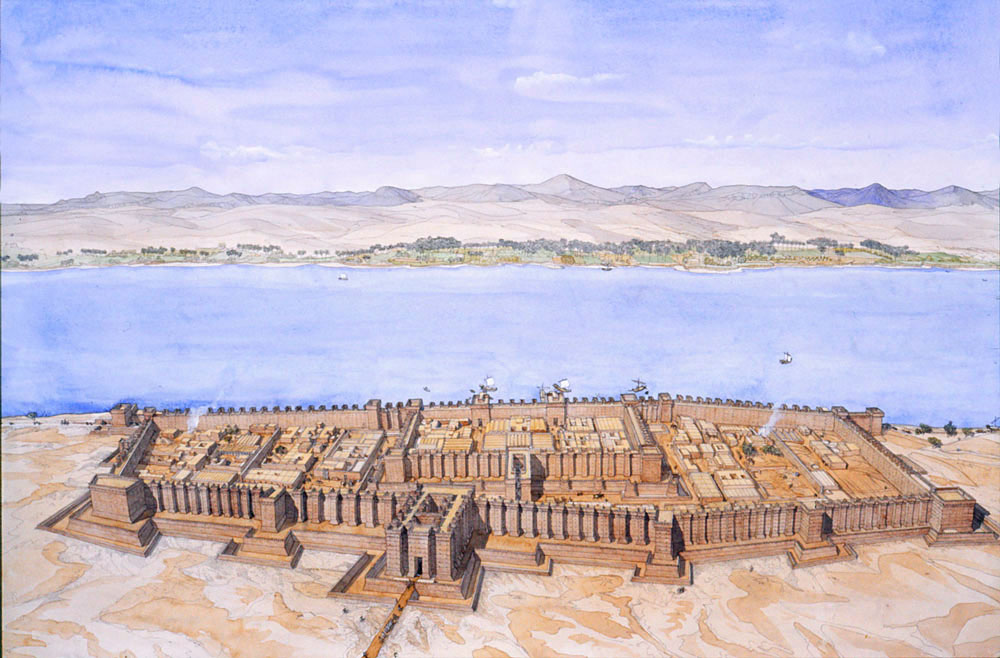
\includegraphics[width=\textwidth]{img/fortress/reconstruction_fortress_of_buhen}
	\caption{Historical reconstruction of the massive Middle Kingdom Egyptian fortress of Buhen, to the north of the 2nd cataract. Although unmistakably Egyptian, this fort fell in to Kushite hands many times since the fall of the Middle Kingdom, and even saw use by the Ptolemies in their Nubian campaigns.}
\end{figure}

Lastly, some explanation behind the walls of the "Royal City", the central walled district of Meroe, and "The Great Enclosure" in Musawwarat es Sufra, from "Hellenizing Art in Ancient Nubia 300 B.C. - AD 250 and Its Egyptian Models", by Laszlo Torok  

%TODO Type in text about Fortification
\begin{figure}[H]
	\centering
	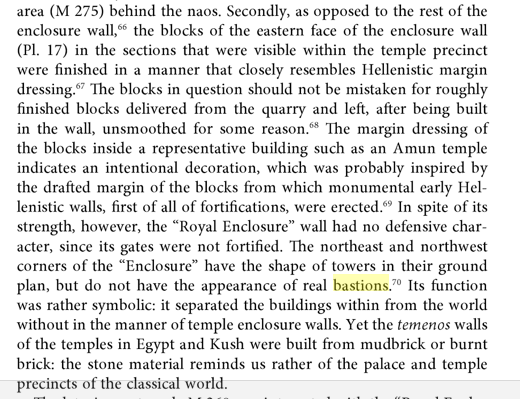
\includegraphics[width=\textwidth]{img/fortress/text_fortification}
	\caption{Text about Fortification}
\end{figure}

\subsection{House}

\paragraph{Status:} 3-D Model Created\\
\paragraph{Phase:} Village\\

\begin{figure}[H]
	\centering
	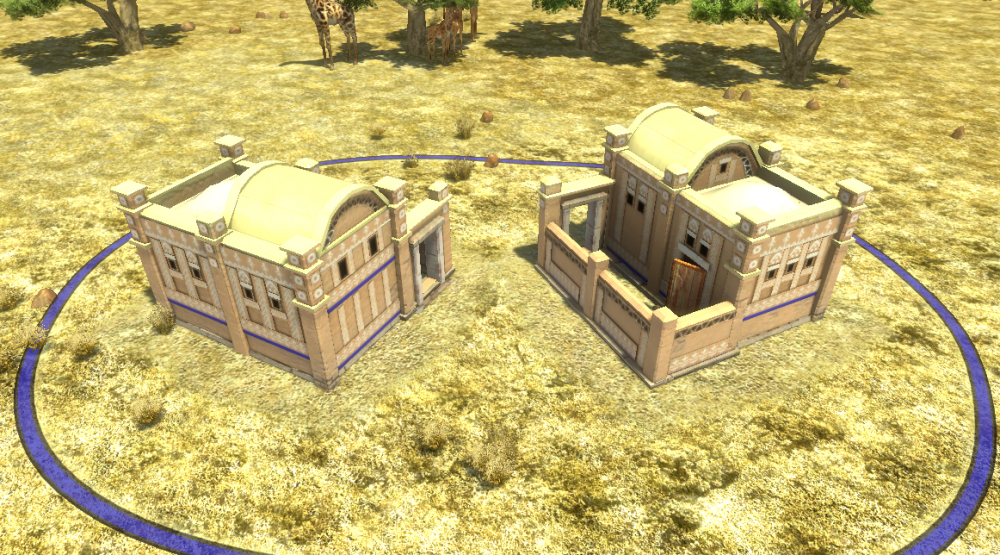
\includegraphics[width=\textwidth]{img/house/house_variation1}
	\caption{3-D model of house variation 1 by @LordGood}
\end{figure}

\begin{figure}[H]
	\centering
	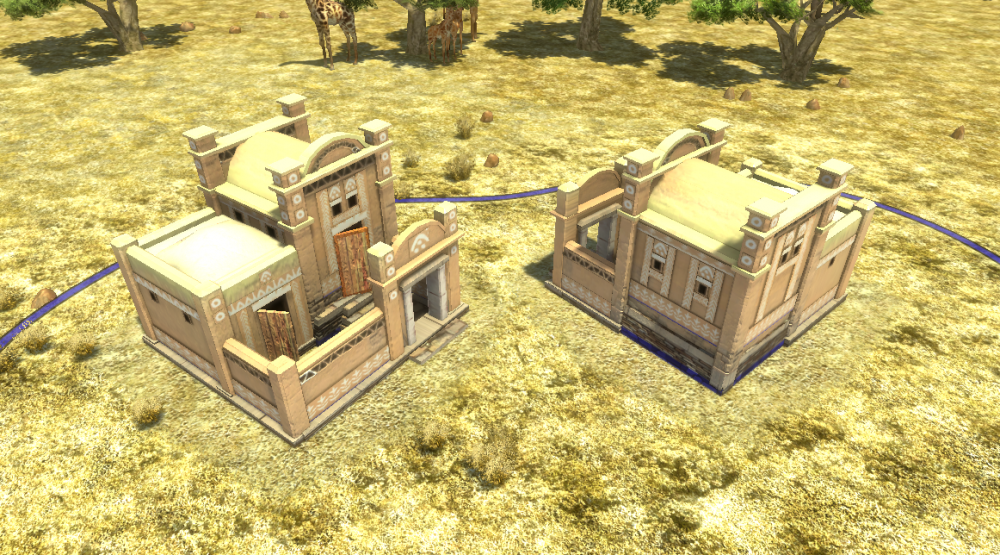
\includegraphics[width=\textwidth]{img/house/house_variation2}
	\caption{3-D model of house variation 2 by @LordGood}
\end{figure}

\begin{figure}[H]
	\centering
	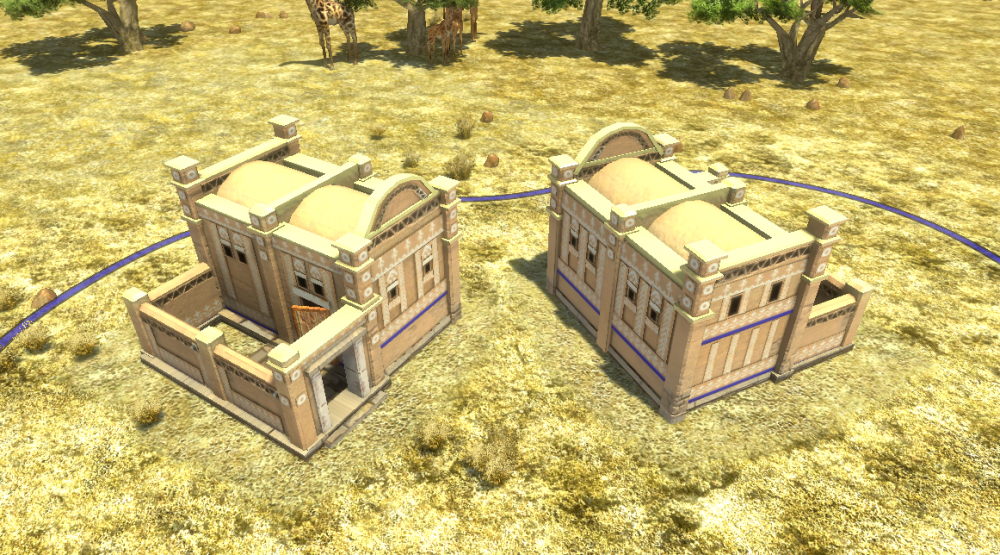
\includegraphics[width=\textwidth]{img/house/house_variation3}
	\caption{3-D model of house variation 3 by @LordGood}
\end{figure}

\begin{figure}[H]
	\centering
	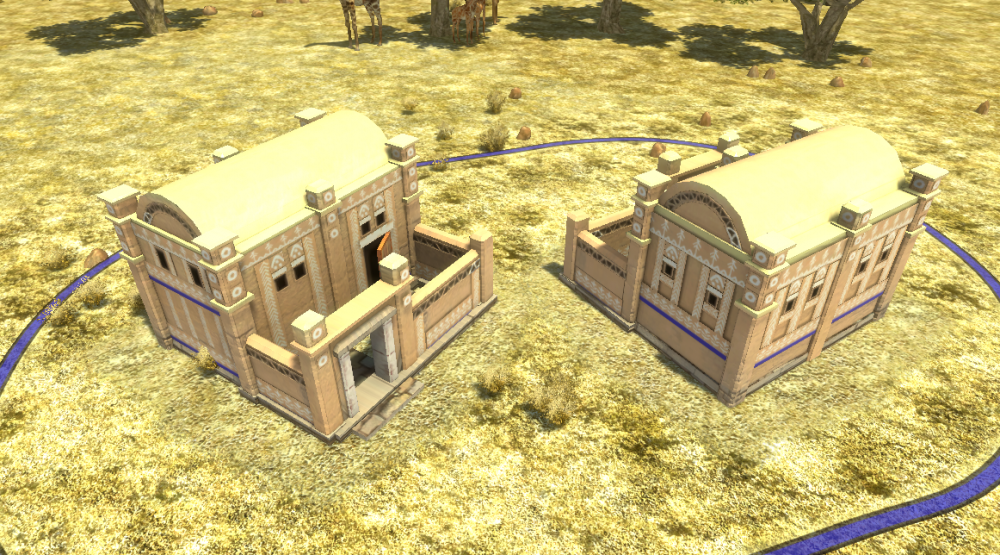
\includegraphics[width=\textwidth]{img/house/house_variation4}
	\caption{3-D model of house variation 4 by @LordGood}
\end{figure}

\begin{figure}[H]
	\centering
	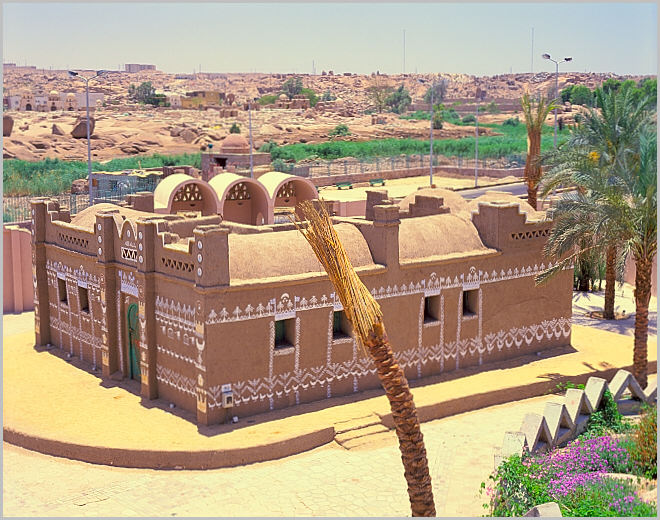
\includegraphics[width=\textwidth]{img/house/recreation_nubian_architecture}
	\caption{A recreation of a meroitic house in the Nubian Museum in Aswan. Rectangular rooms, with vaulted ceilings arranged around a central courtyard. Mud plaster and painted decorations finish the design.}
\end{figure}

\begin{figure}[H]
	\centering
	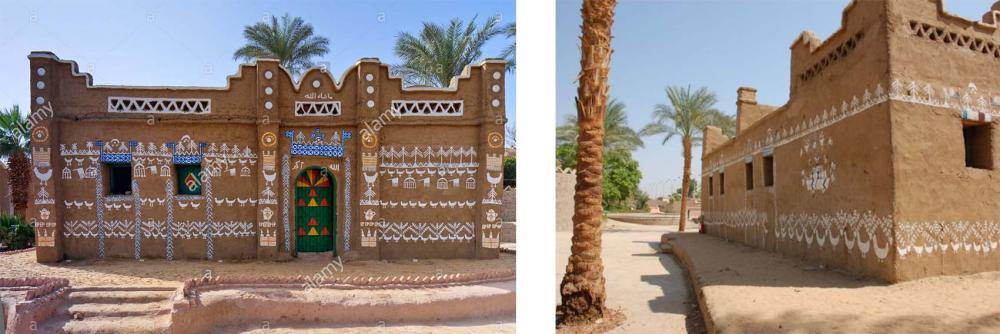
\includegraphics[width=\textwidth]{img/house/nubian_house_museum}
	\caption{Details on a traditional (non-whitewashed) Nubian house in the Nubian Museum, Aswan.}
\end{figure}

\paragraph{About the Common House \ref{fig:common_house}:} Looks quite Kushite. The large ceramic pot, fixed in the floor in the corner of the courtyard is very good. I saw pictures of that in archeological digs of Meroitic sites.\\

Each civ has a number of house models. Kush should also feature this variety. Based on the examples given, maybe 3 or 4 models can be made. For uniformity, they can all be plastered white, with similar geometric designs decorating the spaces around doors and windows. 

\begin{figure}[H]
	\centering
	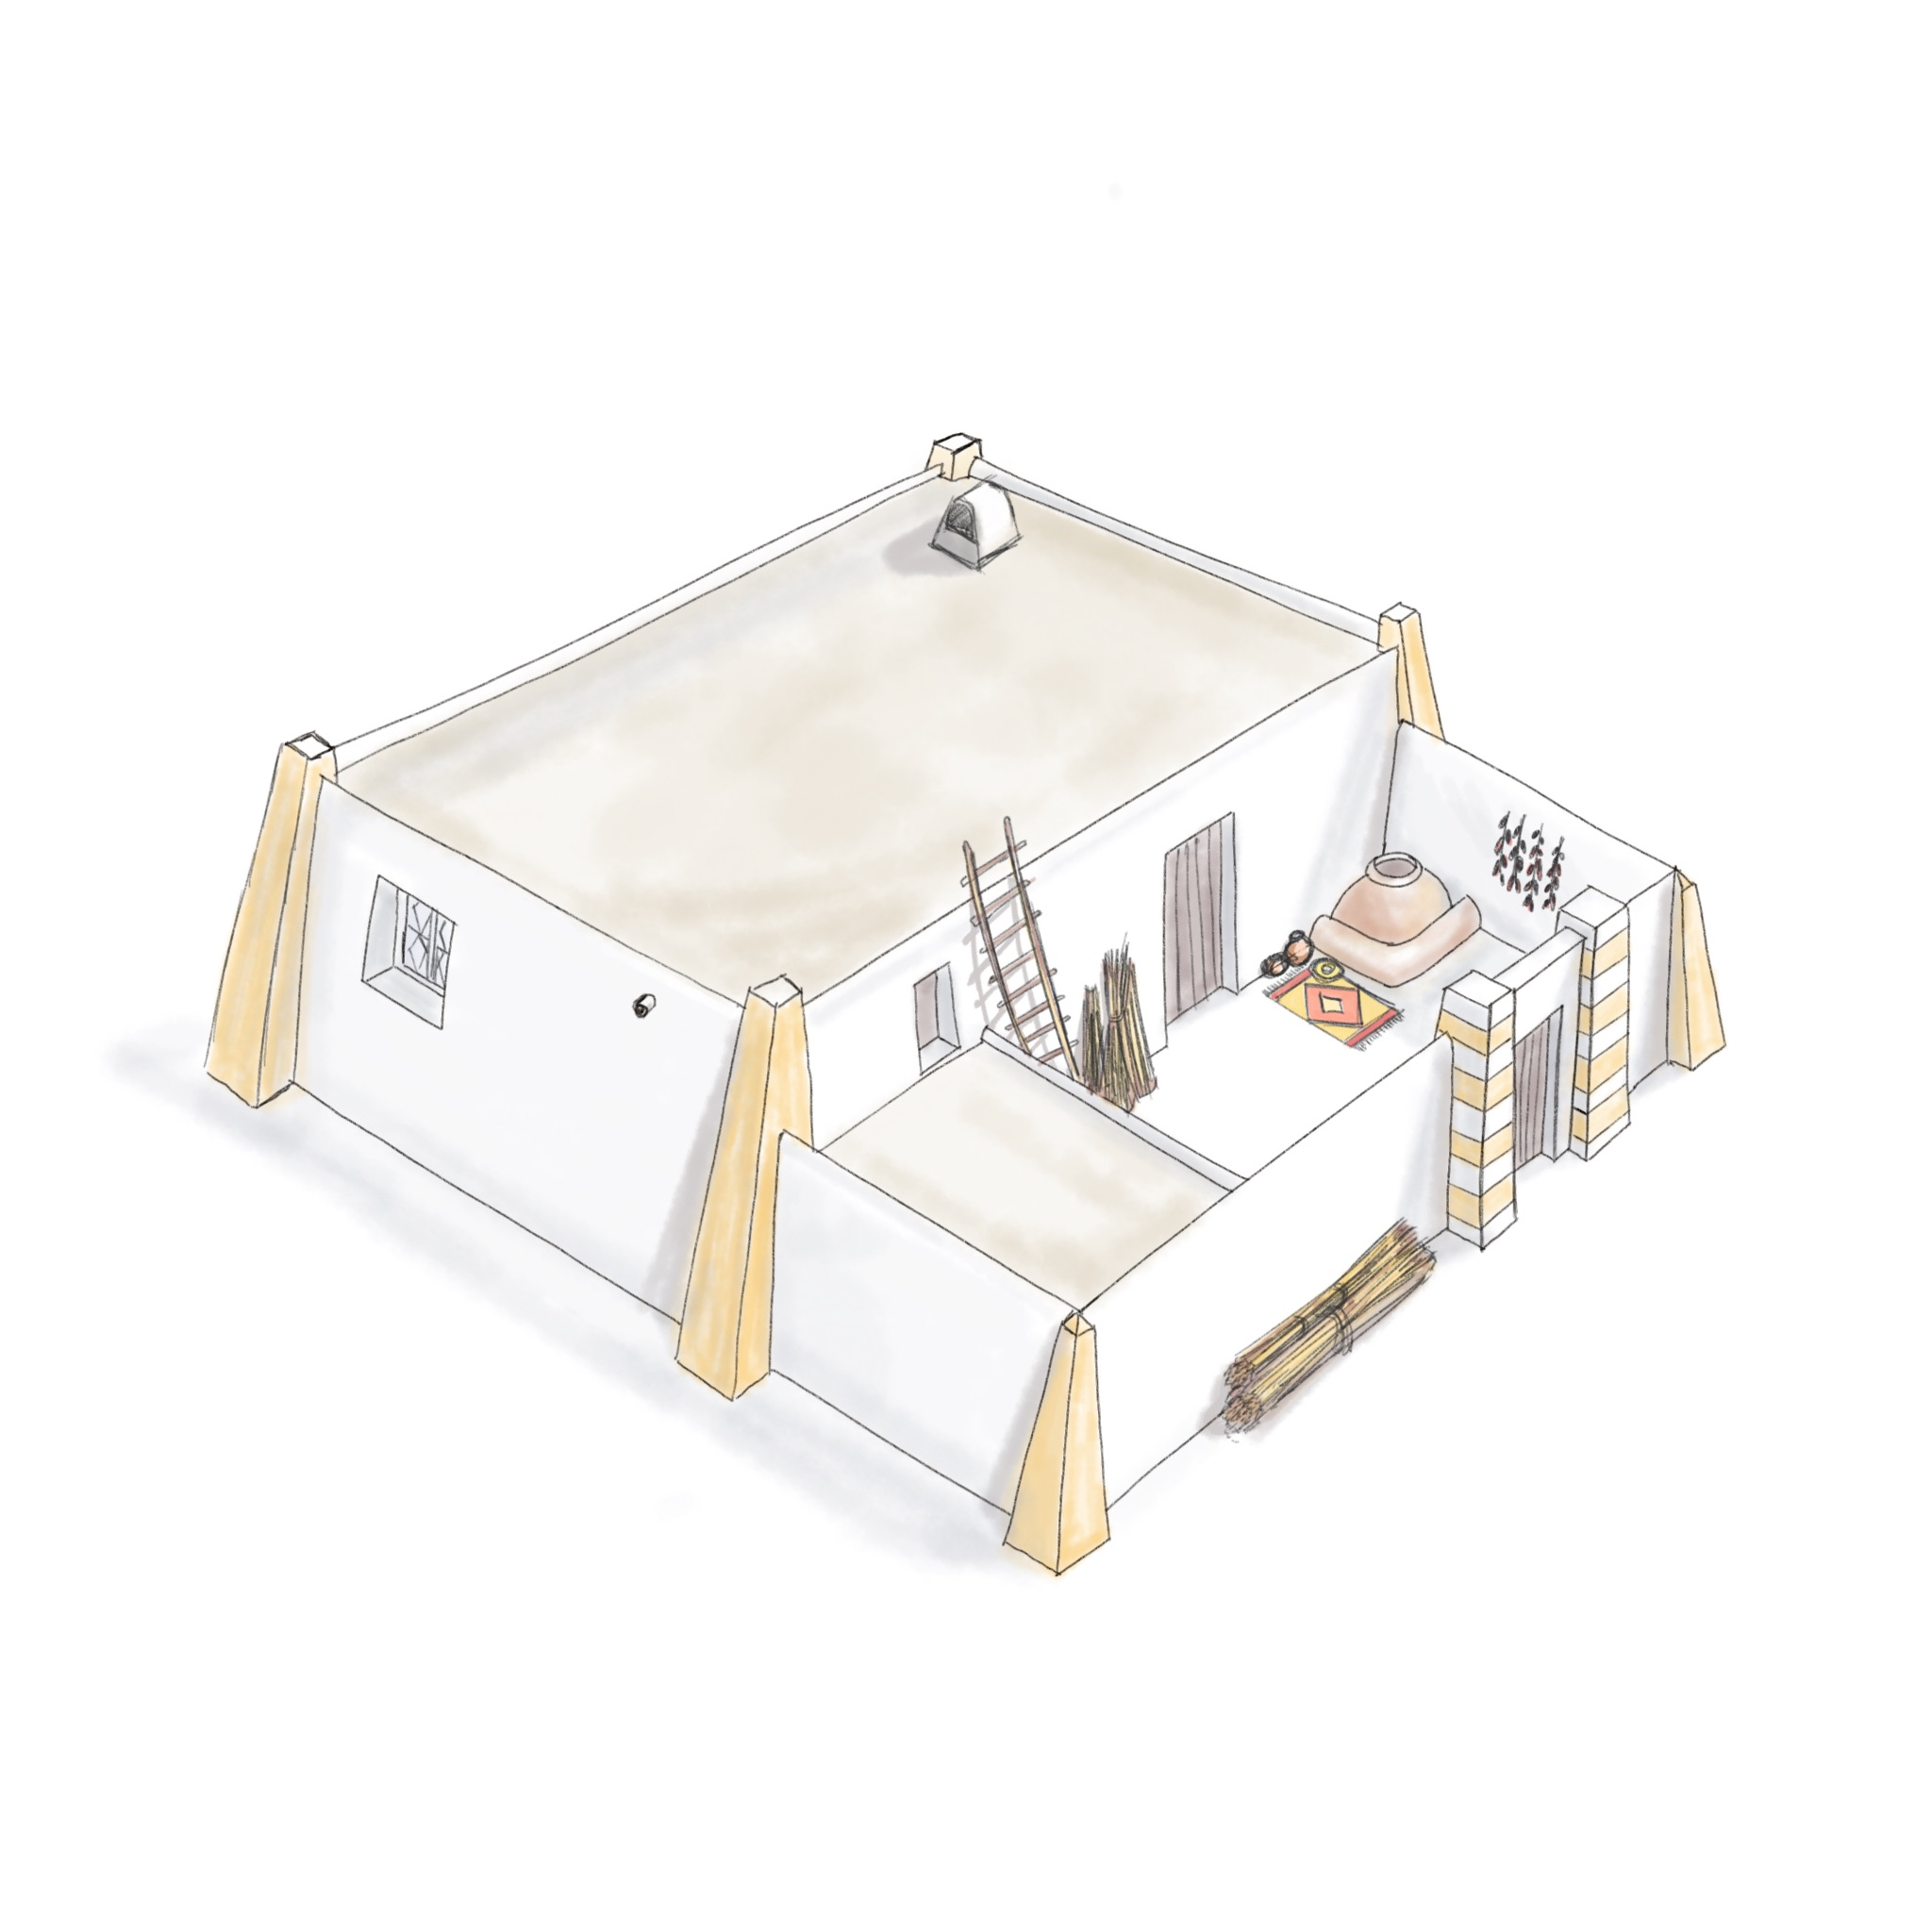
\includegraphics[width=\textwidth]{img/house/juli51_common_house}
	\caption{Common House by @Juli51}\label{fig:common_house}
\end{figure}

\paragraph{About the House Sketch \ref{fig:house_sketch}:} I made a quick sketch of a Meroitic house based on the layout you presented in your second work, "the common house" \ref{fig:common_house}. I adjusted the design, to incorporate Kushitic architectural elements. Like a narrow hall with barrel vault roof. I also made the windows facing outward very small, and placed them high in the wall, so that intruders can't crawl through them. I made the roof of the smaller structure out of palm branches, supported by a light wooden frame. This provides shade, but allows smoke to leave the room, which is how they made their kitchens. It makes for good cooking. I also added some improvised decoration to the front wall 

\begin{figure}[H]
	\centering
	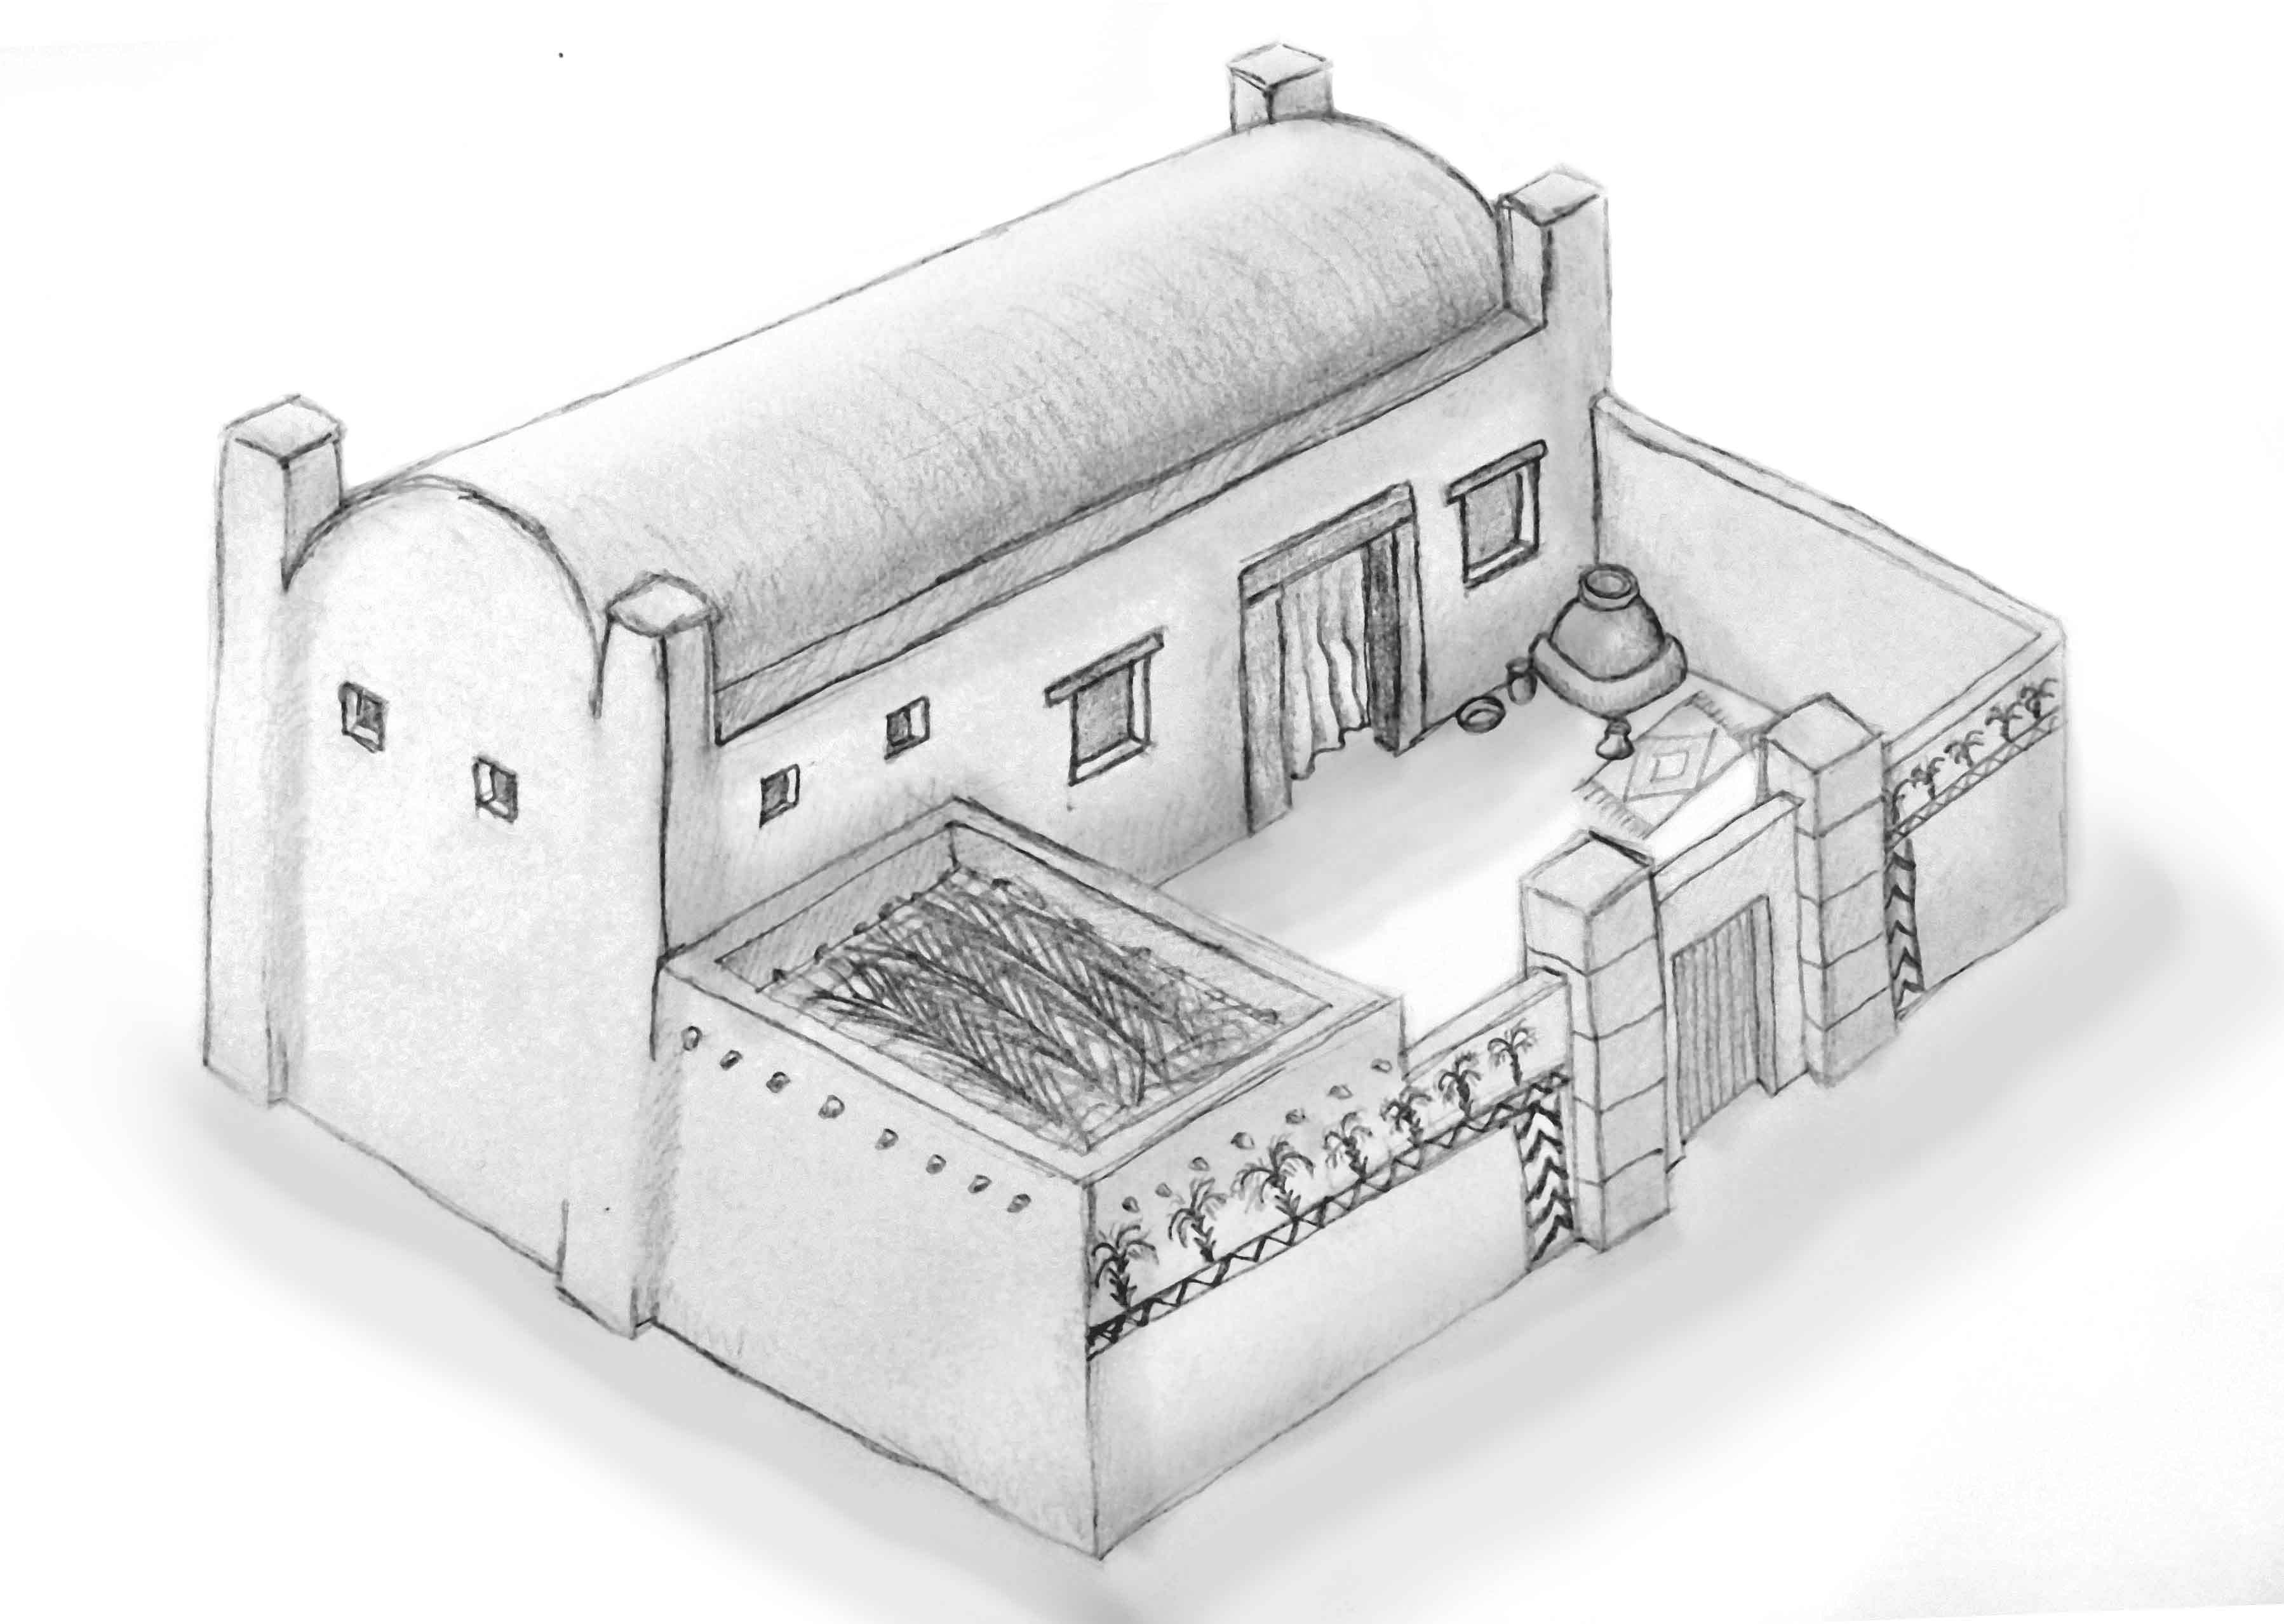
\includegraphics[width=\textwidth]{img/house/sundiata_house_sketch}
	\caption{House Sketch by @Sundiata}\label{fig:house_sketch}
\end{figure}

\begin{figure}[H]
	\centering
	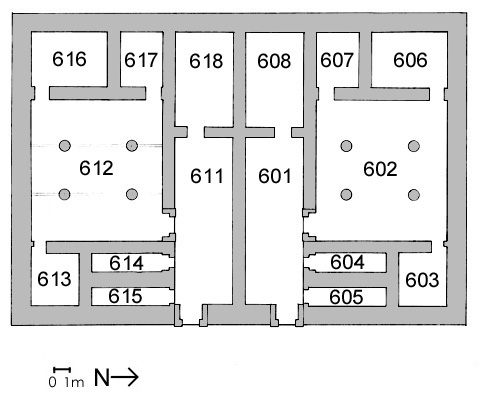
\includegraphics[width=\textwidth]{img/house/meroitic_double_house_floor_plan}
	\caption{Floor plan of a Meroitic double house in Al-Meragh. Two identical halves, but completely separated from each other by a thick dividing wall. This was only one of a number of nearly identical structures in the immediate area.}
\end{figure}

\begin{figure}[H]
	\centering
	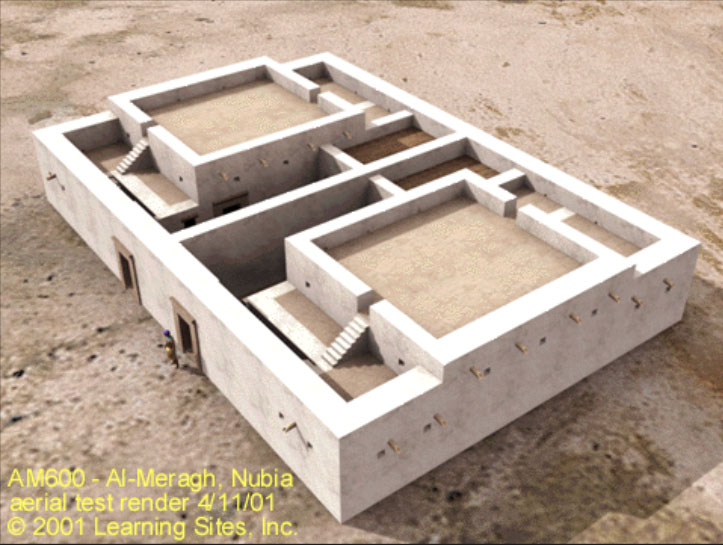
\includegraphics[width=\textwidth]{img/house/3d_model_of_meroitic_double_house}
	\caption{3d rendered model of the Meroitic double house at Al-Meragh. Built with brick, it's doorways were lined with cut stone. The outside of the house received a fine white lime plastering. Stairs leading up to a flat roof, probably used for a variety of purposes.}
\end{figure}

\begin{figure}[H]
	\centering
	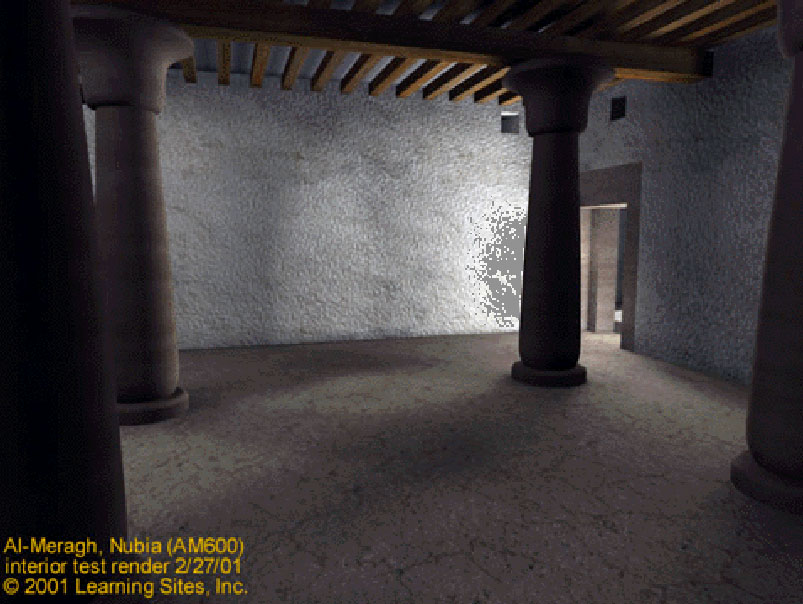
\includegraphics[width=\textwidth]{img/house/double_house_inside}
	\caption{Inside the central living room in one half of the Al-Meragh compound. Stone pillars and capitols support wood beamed roof. Small windows allow for light and air circulation, but they are small enough to keep out unwanted guests.}
\end{figure}

\begin{figure}[H]
	\centering
	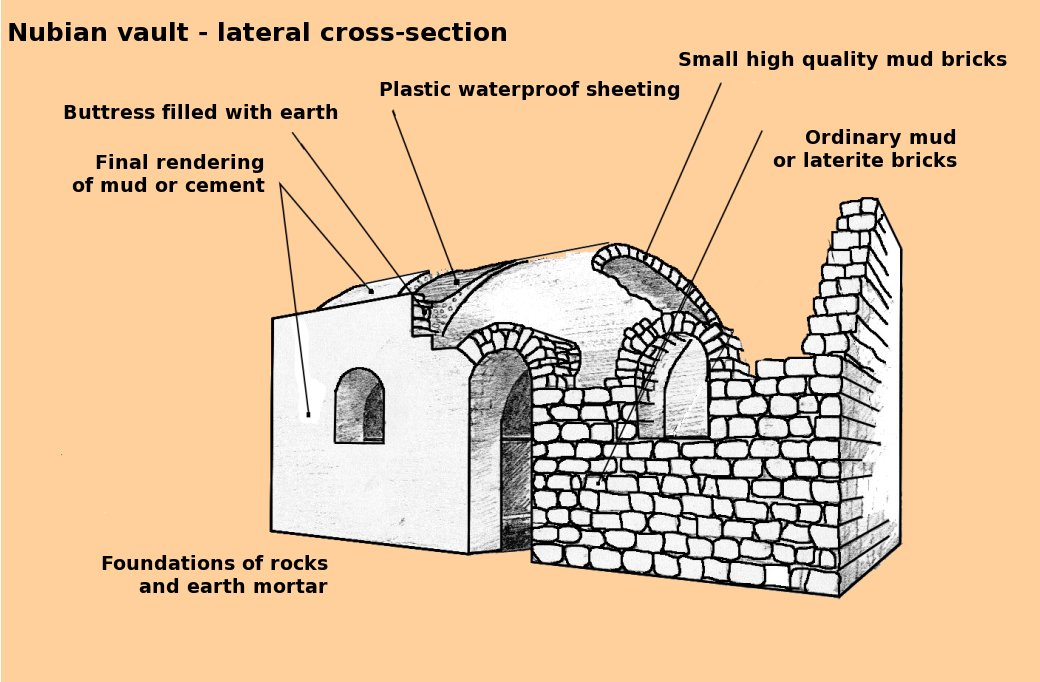
\includegraphics[width=\textwidth]{img/house/nubian_vault_sketch}
	\caption{A modern example of an ancient design. Featuring the Nubian vault and arched windows. Many common houses in Meroitic Kush would have looked identical to this one.}
\end{figure}

\subsection{Market}

%TODO market should have tends and fruits (should be more colorful)
%no palm trees and other stuff

\begin{figure}[H]
	\centering
	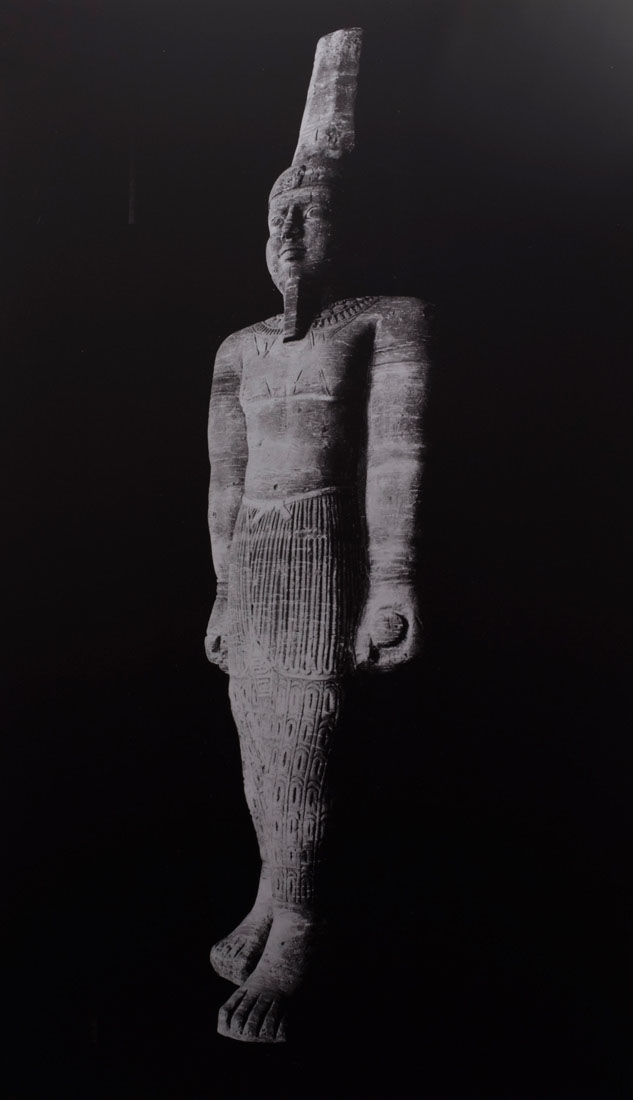
\includegraphics[width=\textwidth]{img/market/arensnuphis_statue}
	\caption{Arensnuphis, a Kushite deity}
\end{figure}

\subsection{Temple}

\paragraph{Phase:} Town\\

With the move to Meroe, a local South Nubian deity, known as Apedemak, rose to prominence. This lion headed god of war might have even eclipsed the worship of Amun. During the Meroitic period, many new temples were built, in Napata, Naqa, Wad Ben Naqa, Musawwarat es Sufra, Hamadab, Dangeil and other important centers. Usually to Amun or Apedemak, but also to Hathor and Isis, and some temples and shrines were also dedicated to lesser-known Nubian gods. Although stylistically still Egyptian, the floor plan of these temples was typically Kushite. 

\begin{figure}[H]
	\centering
	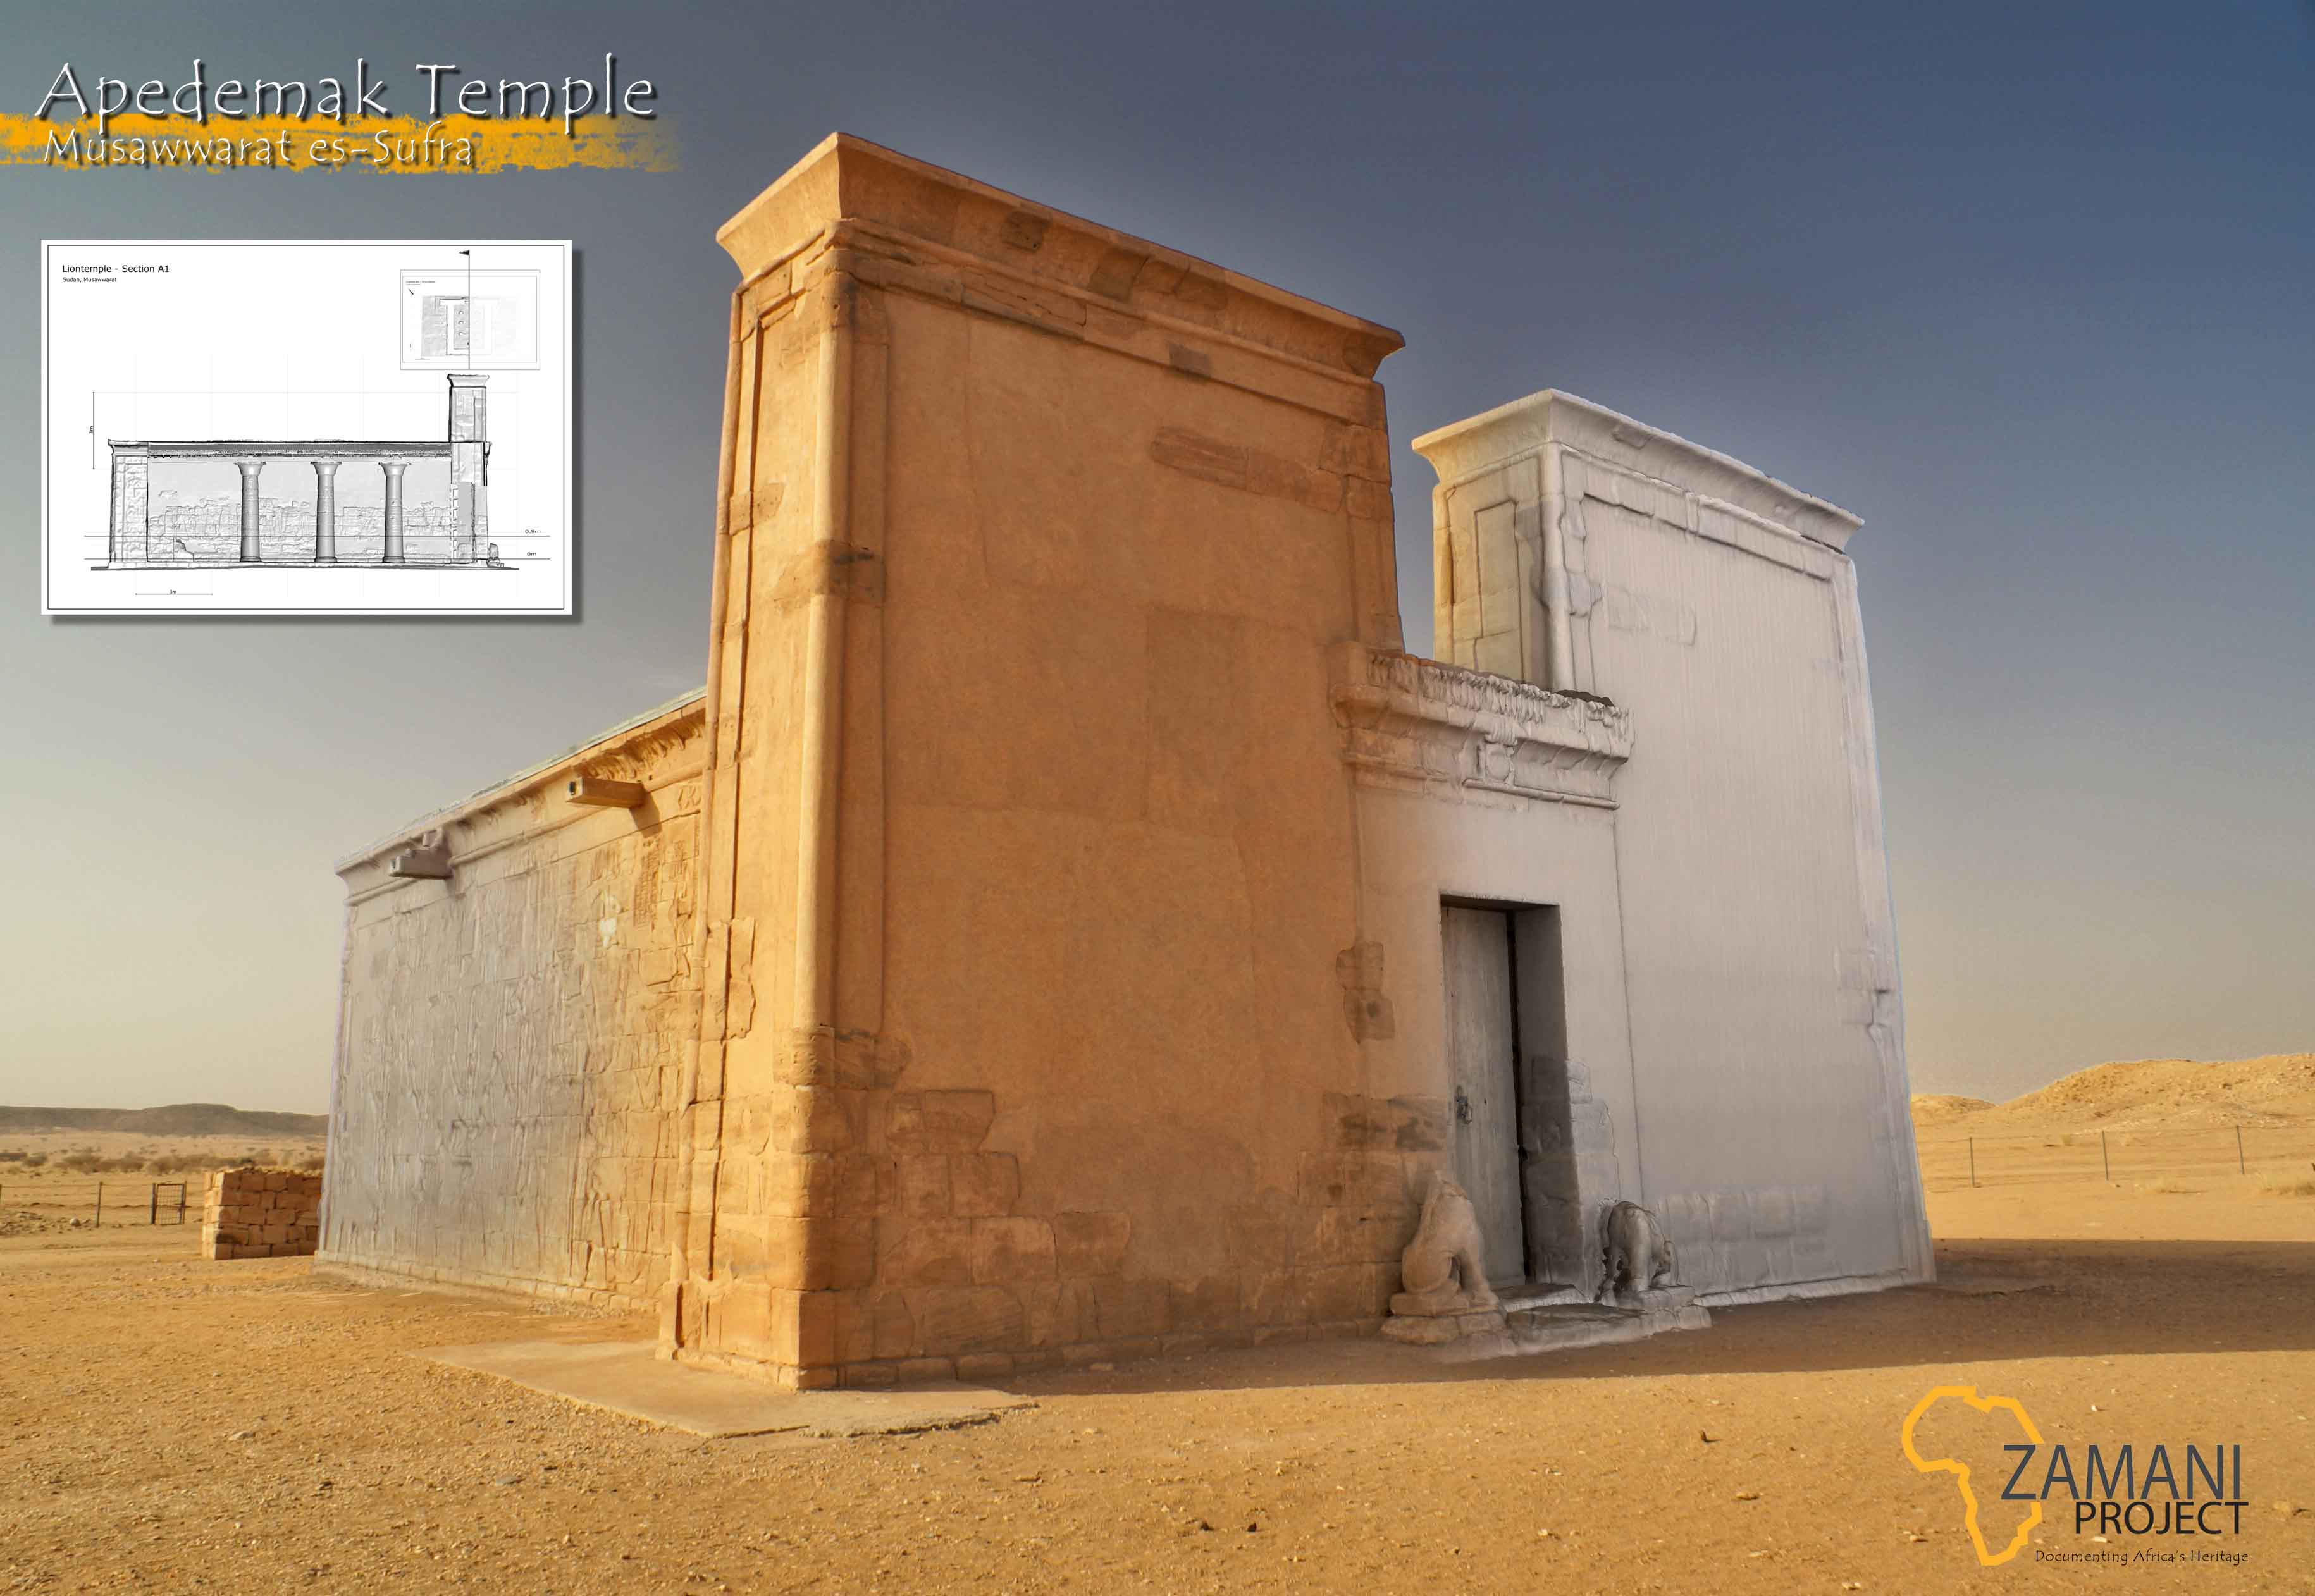
\includegraphics[width=\textwidth]{img/temple/apedemak_temple}
	\caption{A beautiful example of a temple to Apedemak, Musawwarat es Sufra}
\end{figure}

\begin{figure}[H]
	\centering
	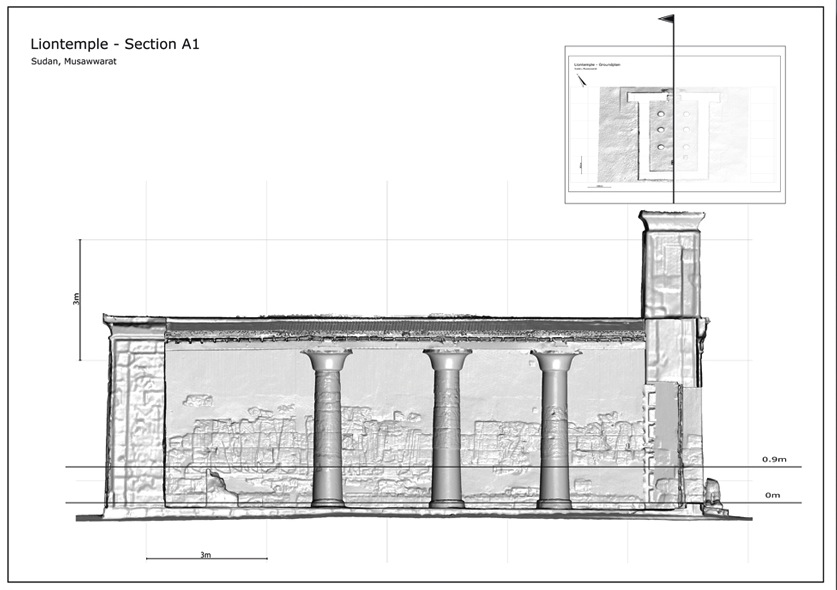
\includegraphics[width=\textwidth]{img/temple/apedemak_temple_profile}
	\caption{Temple to Apedemak, the lion headed god of war, in Musawwarat es Sufra}
\end{figure}

\subsection{Wall + Gates}

Kushites used a variety of techniques to build walls, and yes, they were quite good at it. Cut stone, dry-stone walls, mudbrick and fired brick were all used to varying degrees depending on the site you’re examining. These building materials were also used extensively in combination with each other. Some walls were built with a social/ritual/religious purpose, separating lower classes from higher classes. Separating the holy of holies from the unholy. In other places they served a purely defensive purpose, with walls that could be manned, and featured bastions.

\begin{figure}[H]
	\centering
	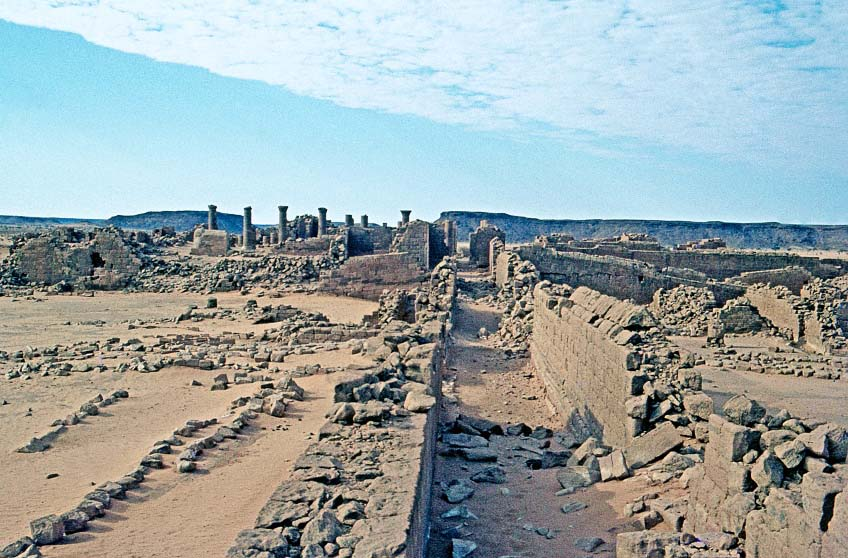
\includegraphics[width=\textwidth]{img/walls_gates/impression_of_wall}
	\caption{Some of the walls that form "the great enclosure" at Musawwarat es Sufra, a religious complex. They give a good impression of Kushite masonry skills. Tightly cut (usually sandstone) blocks, dress the interior section of the wall, made of rubble and uncut stone.}
\end{figure}

\begin{figure}[H]
	\centering
	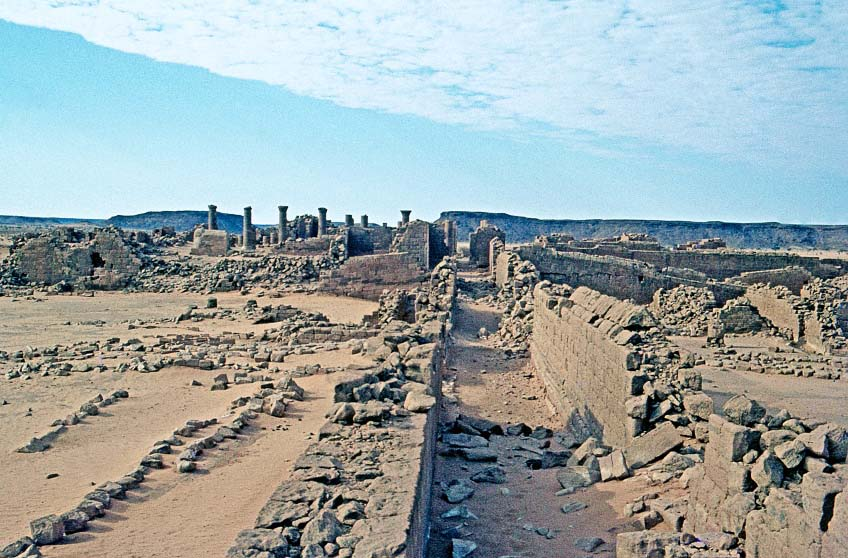
\includegraphics[width=\textwidth]{img/walls_gates/impression_of_wall}
	\caption{Cerimonial walls in Musawwarat es Sufra }
\end{figure}

\begin{figure}[H]
	\centering
	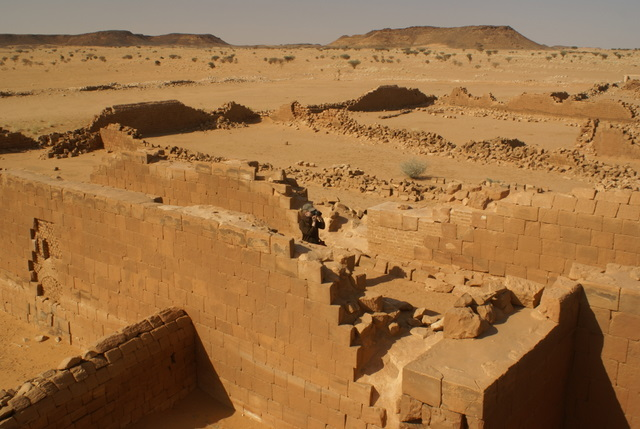
\includegraphics[width=\textwidth]{img/walls_gates/cermonial_wall}
	\caption{Cerimonial walls in Musawwarat es Sufra}
\end{figure}

\begin{figure}[H]
	\centering
	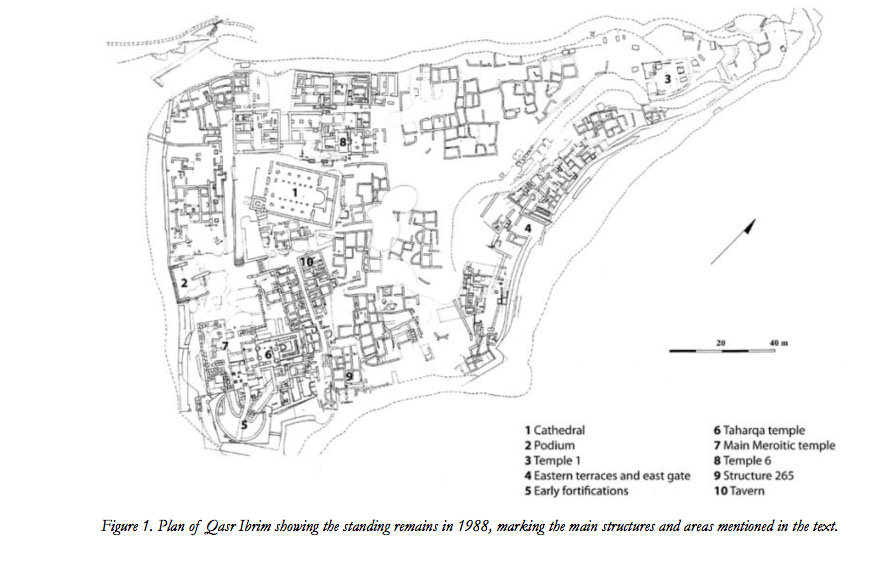
\includegraphics[width=\textwidth]{img/walls_gates/qasr_ibrim_walled_city}
	\caption{Plan of the walled city of Qasr Ibrim, showing remnants from many different eras, including the Christian era cathedral, and the "Taharqa temple". In Meroitic times, it was called Premnis, and formed a battleground for the invading Romans who occupied, and then ceded it back to Kush.}
\end{figure}

An important characteristics of the kushites are the narrow entrance gates.

\begin{figure}[H]
	\centering
	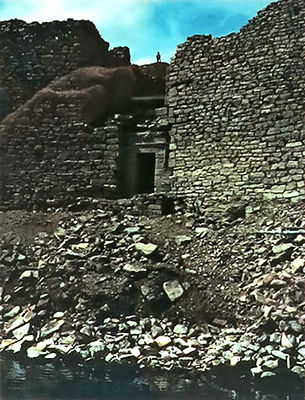
\includegraphics[width=\textwidth]{img/walls_gates/qasr_ibrim_gate}
	\caption{Kushite style, narrow entrance gate to Qasr Ibrim.}
\end{figure}

\begin{figure}[H]
	\centering
	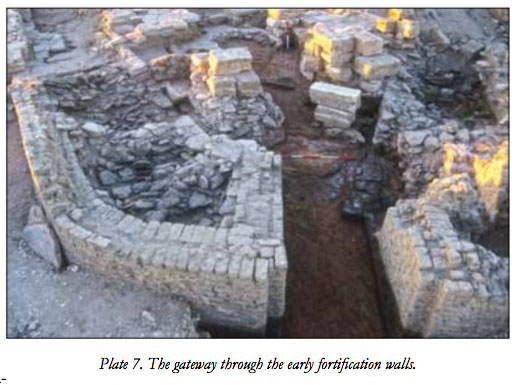
\includegraphics[width=\textwidth]{img/walls_gates/new_kingdom_entrance_gate}
	\caption{New Kingdom entrance gate to Qasr Ibrim, rebuilt and narrowed during later (possibly Meroitic) times.}
\end{figure}

\subsubsection{Low Wall}

\paragraph{Phase:} Village\\



\subsubsection{Low Wall Gate}

\paragraph{Phase:} Village\\

\subsubsection{City Wall}

\paragraph{Phase:} Town\\

The Kushites knew how to build massive walls. The central part of Meroe was surrounded by a city wall with a thickness from 3,5 - 7,75 m. The entire city wall was made from dressed stone. Even today, some of the remains of the city wall are 3,5 m in height \citep[p. 43]{welsby_kingdom_2005}.

\subsubsection{City Gate}

\paragraph{Phase:} Town\\

\subsection{Wonder}

\paragraph{Phase:} City\\

The Meroitic pyramids would be a good wonder. They’re not awkwardly big, but still imposing enough, and built with an eastward facing chapel, they have an interesting architectural element.

\begin{figure}[H]
	\centering
	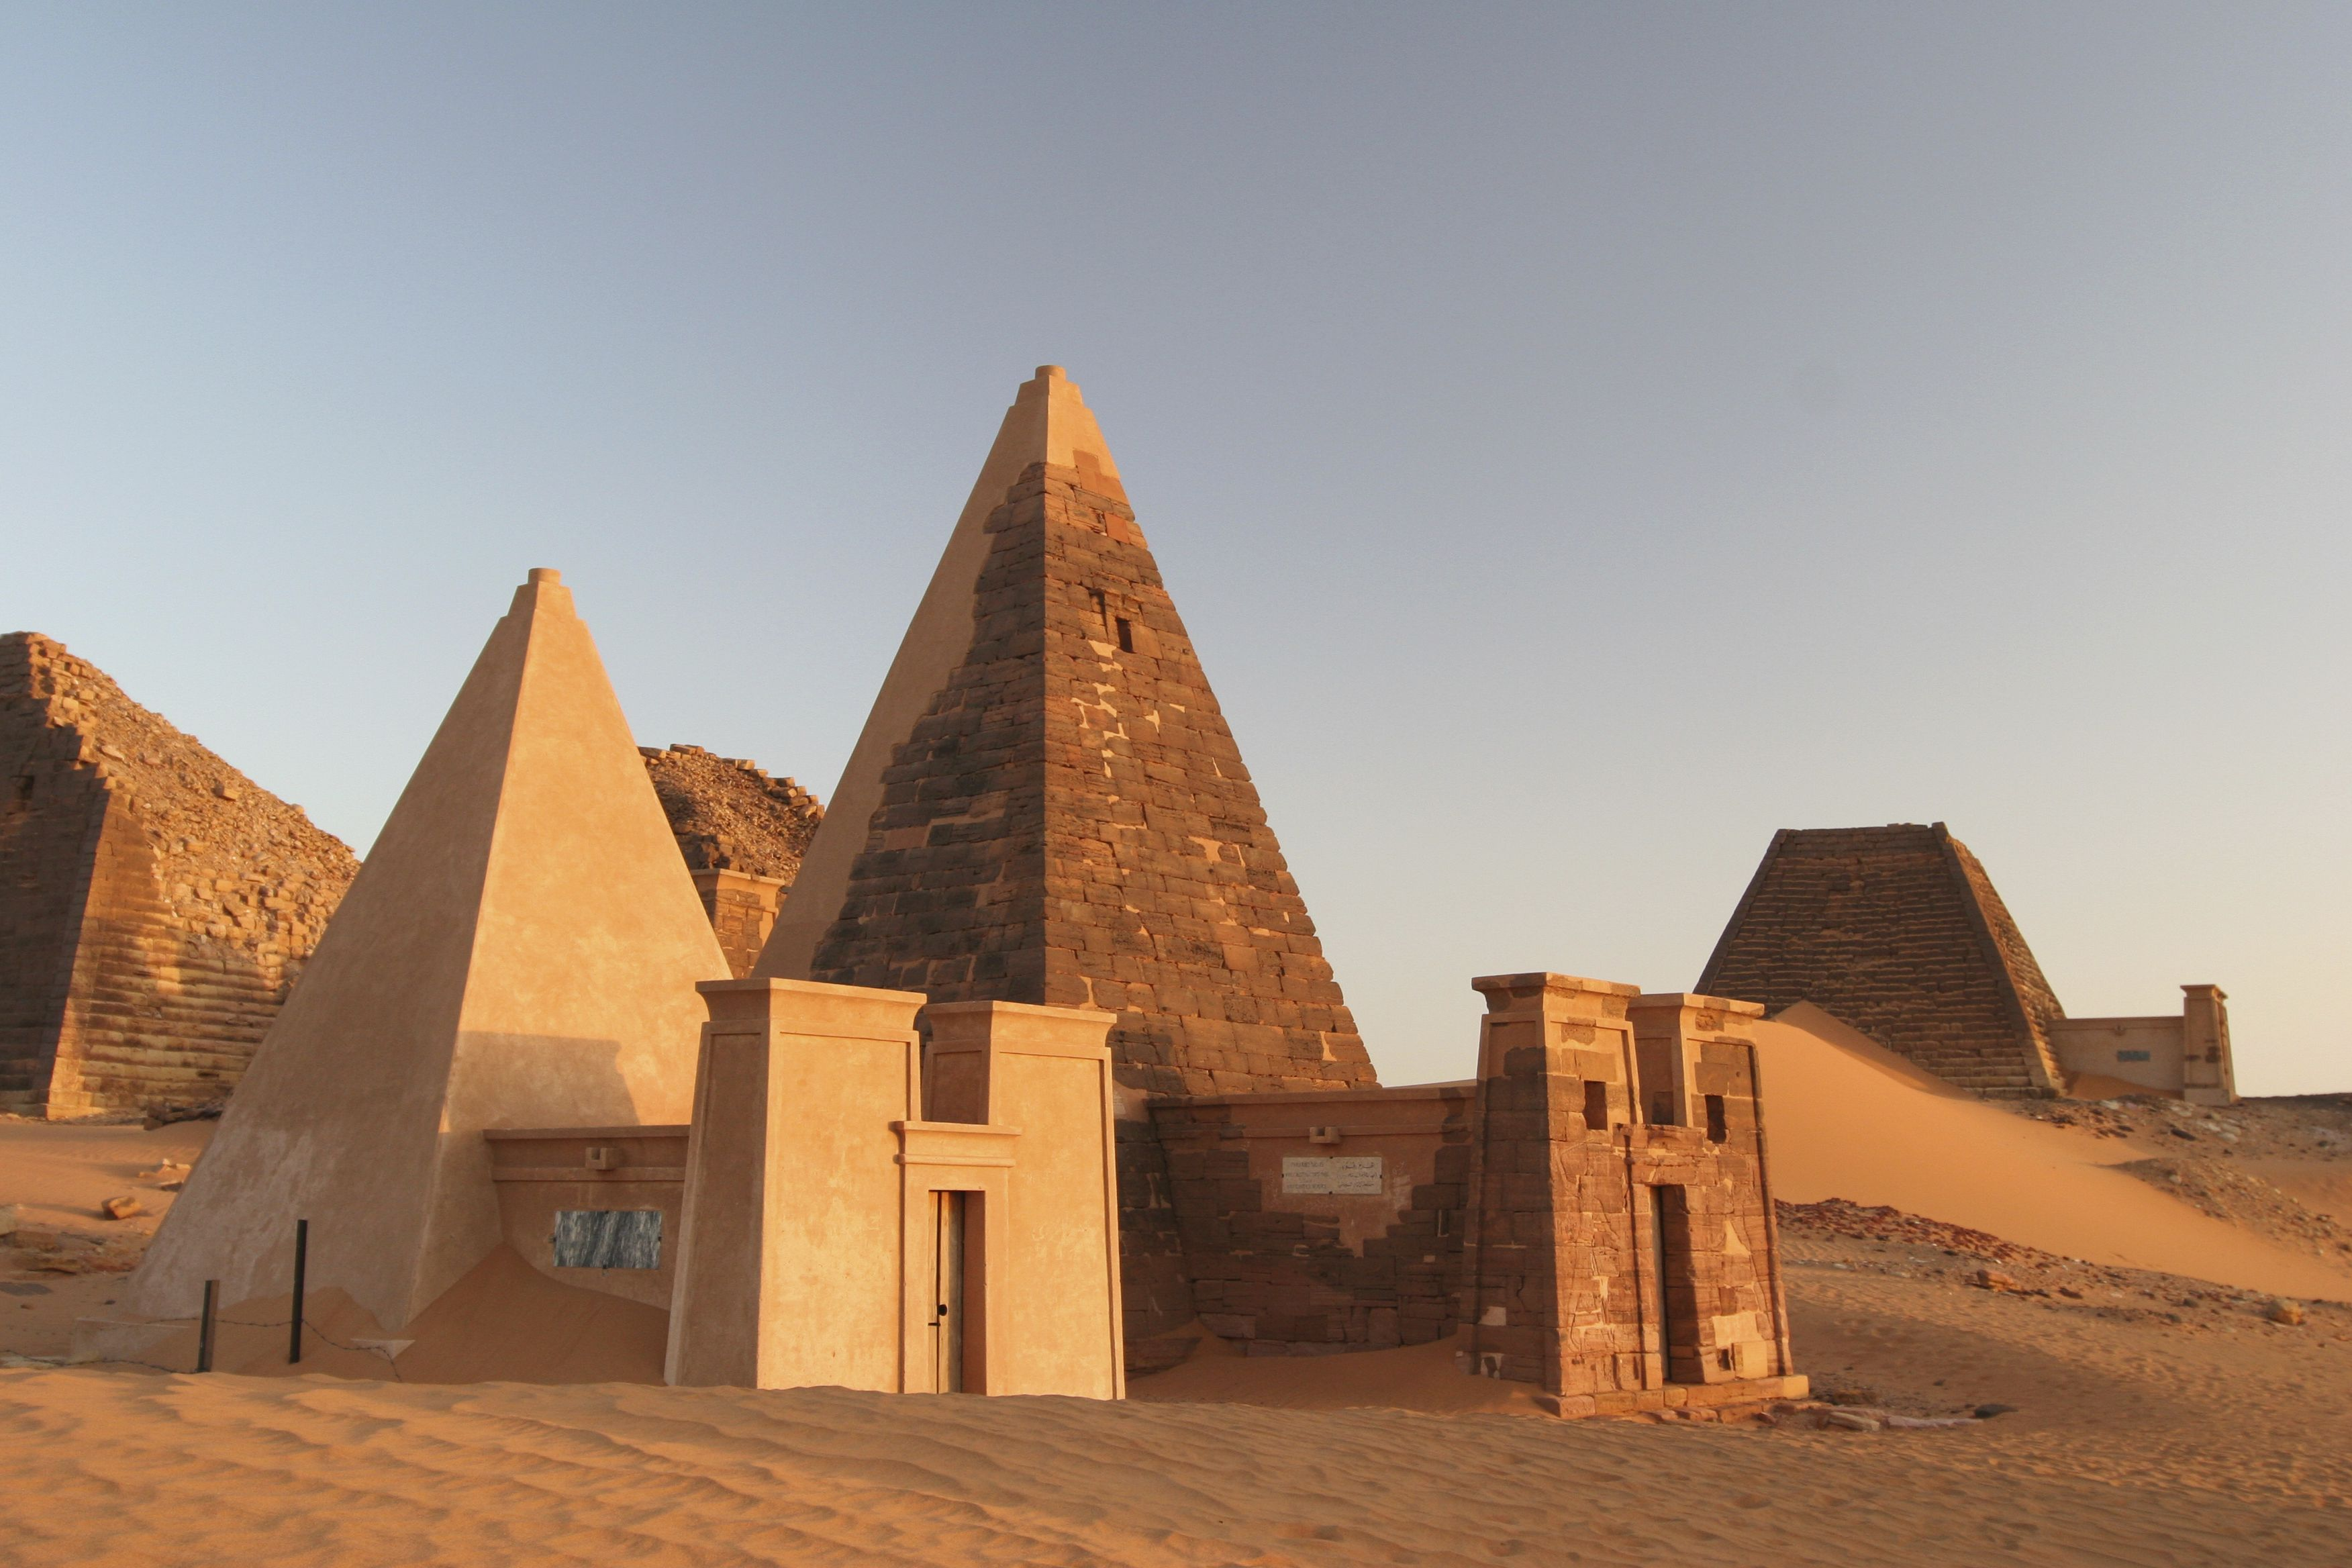
\includegraphics[width=\textwidth]{img/wonder/nubian_pyramids_original}
	\caption{Pyramids from \url{http://www.thousandwonders.net/}}
\end{figure}

\begin{figure}[H]
	\centering
	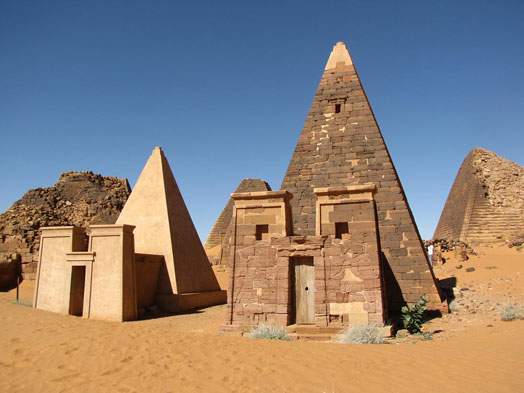
\includegraphics[width=\textwidth]{img/wonder/meroe-pyramids}
	\caption{Pyramids front perspective from \url{http://bcarchaeology.com/}}
\end{figure}

\section{Units}

\subsection{Beja}

I think Beja tribesmen (Blemmyes), would serve as ideal mercenary units. Beja were traditional enemies, vassals and overlords of Kush at various times. A strong sword infantry unit, and a camel unit with lance (and perhaps javelins) would be nice compliments to the Kushite unit roster.

\begin{figure}[H]
	\centering
	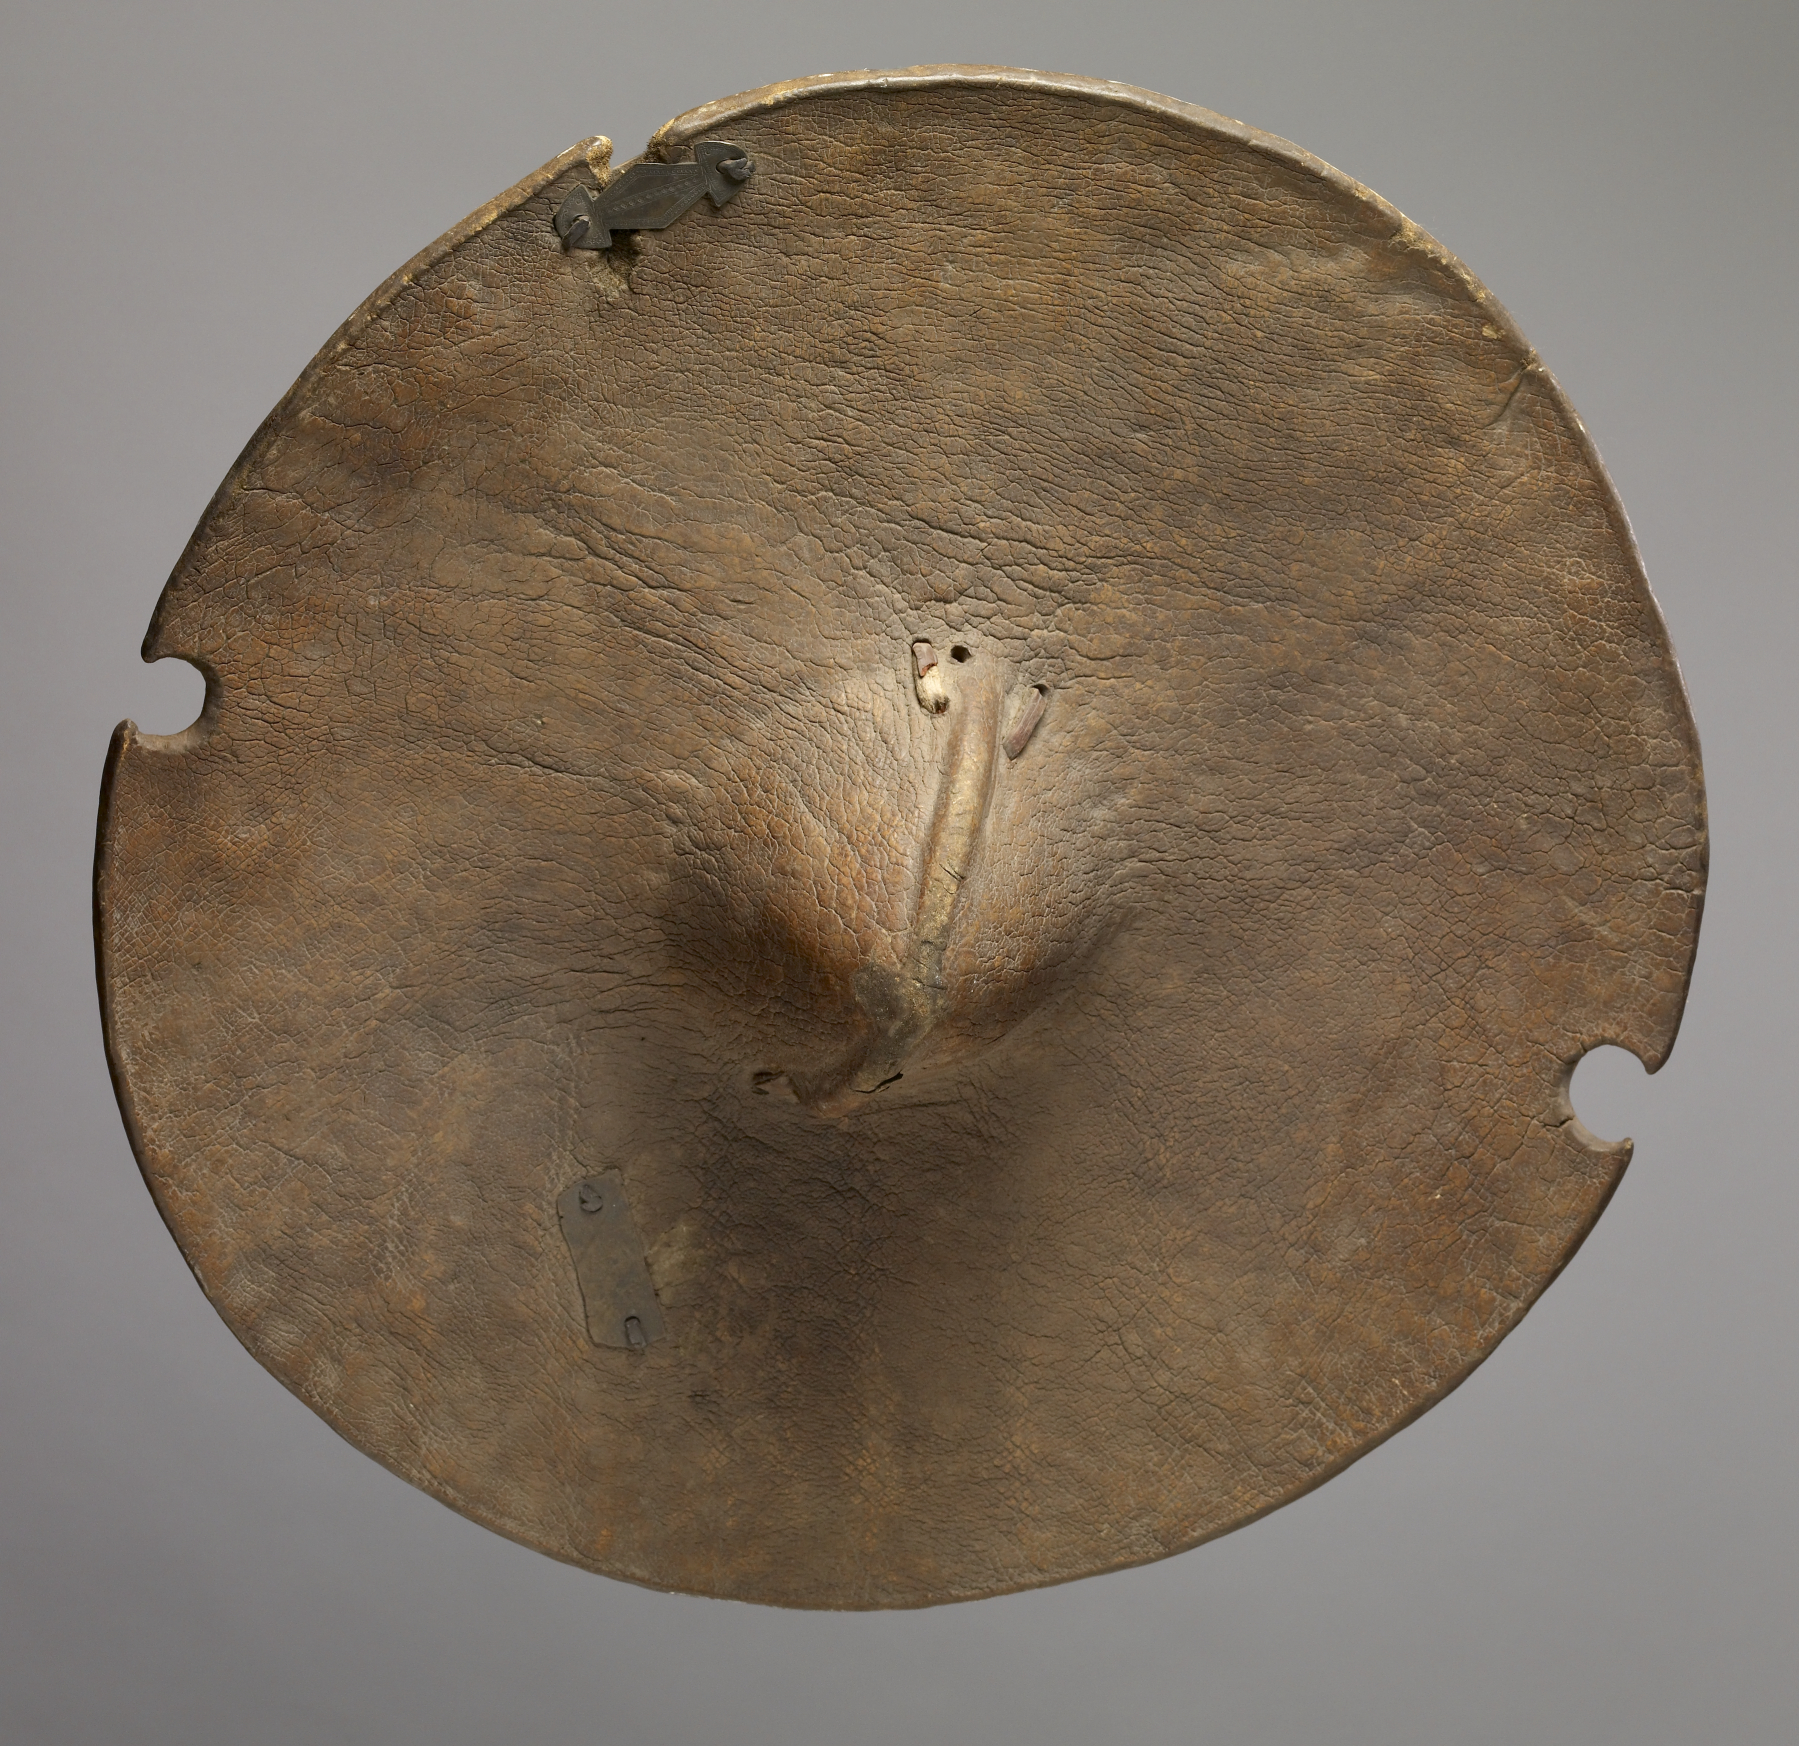
\includegraphics[width=\textwidth]{img/beja/Beja_Shield}
	\caption{A Beja shield made of animal hide from the 20th century. In the collection of the Walters Art Museum. \url{https://en.wikipedia.org/wiki/Beja_people}}
\end{figure}

\subsubsection{Beja Swordsman}

\begin{figure}[H]
	\centering
	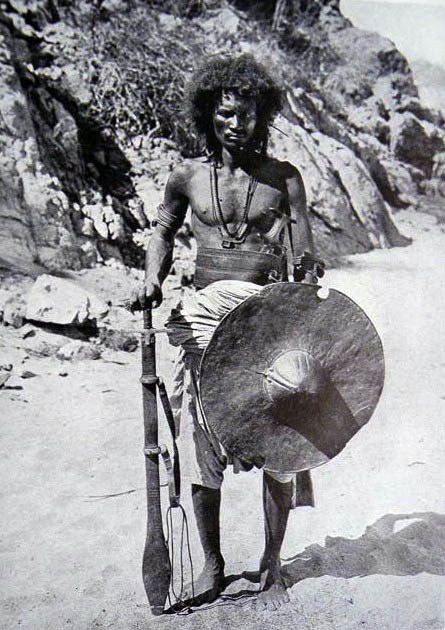
\includegraphics[width=\textwidth]{img/beja/beja_swordsman}
	\caption{A typical Beja swordsman, wearing a white loincloth, animal hide round shield, and dagger tucked away in a broad leather belt protecting his abdomen. I believe the material culture presented in this picture is identical to that of the Meroitic times. Even the shape of the swords' scabbard is a strong reminder of the earlier Kushite Kings and their swords.}
\end{figure}

\subsubsection{Beja Spearman}

\begin{figure}[H]
	\centering
	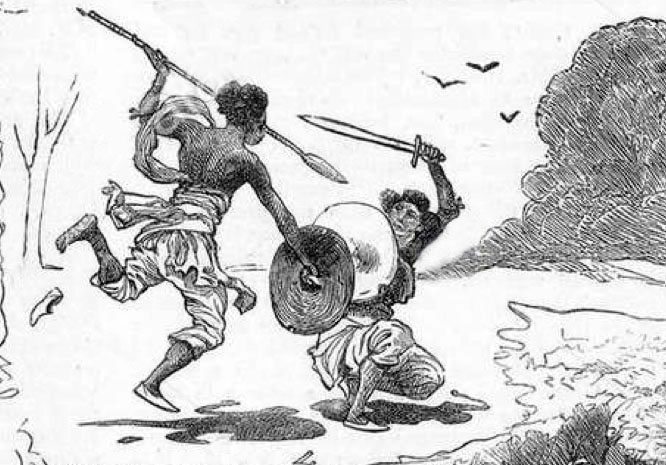
\includegraphics[width=\textwidth]{img/beja/beja_swords_and_spearman}
	\caption{Beja swordsman and spearman sparring. Beja swordsmen form ideal mercenary units.}
\end{figure}

\subsubsection{Beja Camel Warrior}

\begin{figure}[H]
	\centering
	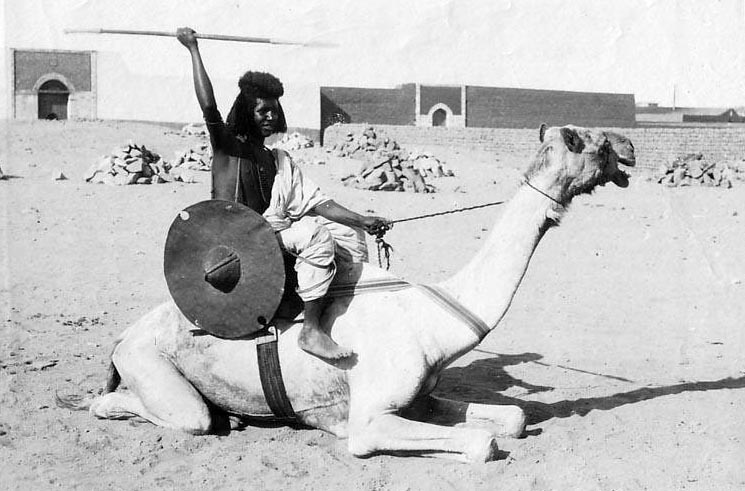
\includegraphics[width=\textwidth]{img/beja/beja_camel_warrior}
	\caption{A Beja camel warrior.}
\end{figure}

\begin{figure}[H]
	\centering
	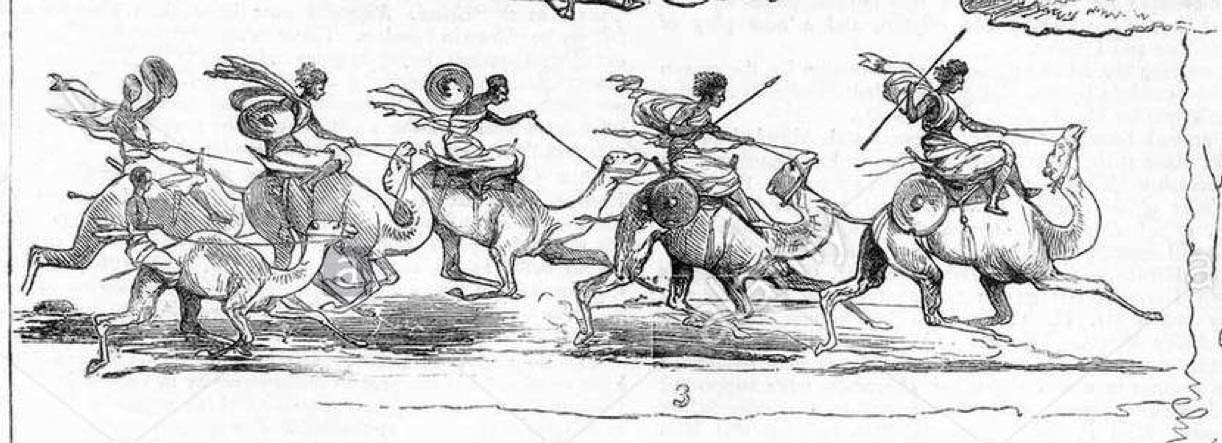
\includegraphics[width=\textwidth]{img/beja/beja_camel_warriors}
	\caption{Beja camel-warriors, equipped with typical round shield and lance.}
\end{figure}

\subsection{Fishing Boat}

\subsection{Meroitic Cavalry}

\subsection{Nubian Bowmen}

\subsection{Priest}

Fig. \ref{fig:taharqa} shows us Taharqa leading a religious procession in Napata. He’s actually wearing the traditional outfit of a high-priest (A white loincloth with a leopard skin draped across his chest, with the leopards’ head dangling at the height of his lower belly/crotch area). On the left side, in front of the chariot, another priest is seen in the same outfit, but without royal regalia.

\begin{figure}[H]
	\centering
	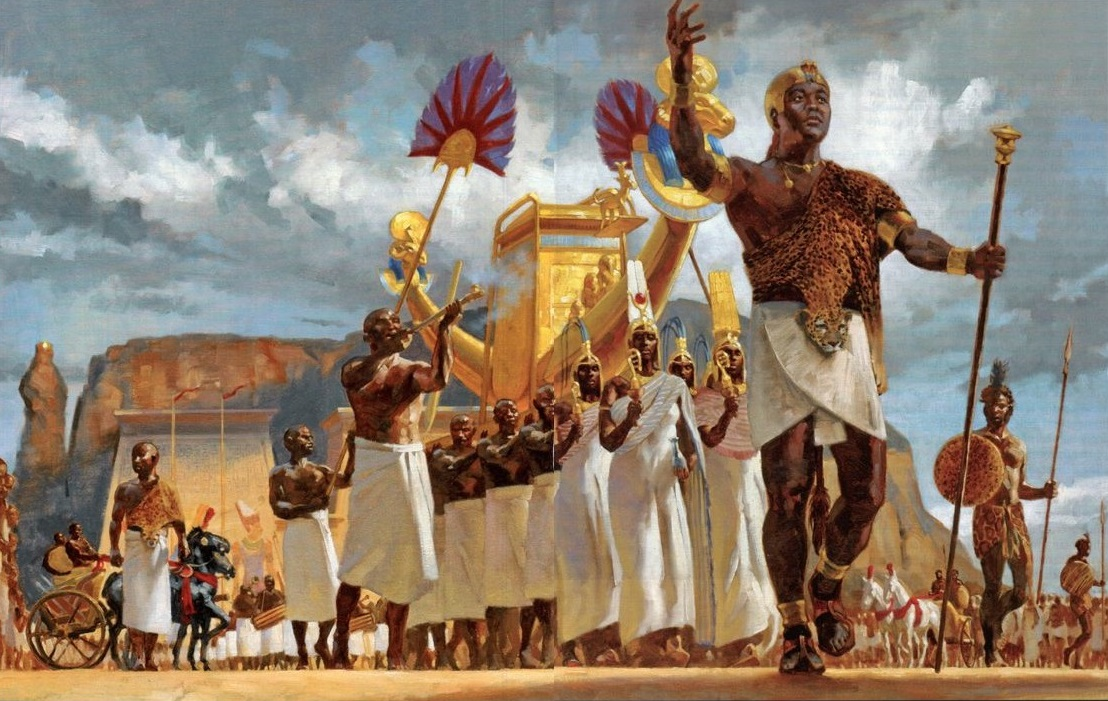
\includegraphics[width=\textwidth]{img/taharqa_pharaoh}
	\caption{Taharqa, pharaoh of the 25th dynasty and father of the later Meroe period, at the temple of Amun in Napata. The holy mountain Jebel (Gebel) Barkal is in the background.}\label{fig:taharqa}
\end{figure}

\begin{figure}[H]
	\centering
	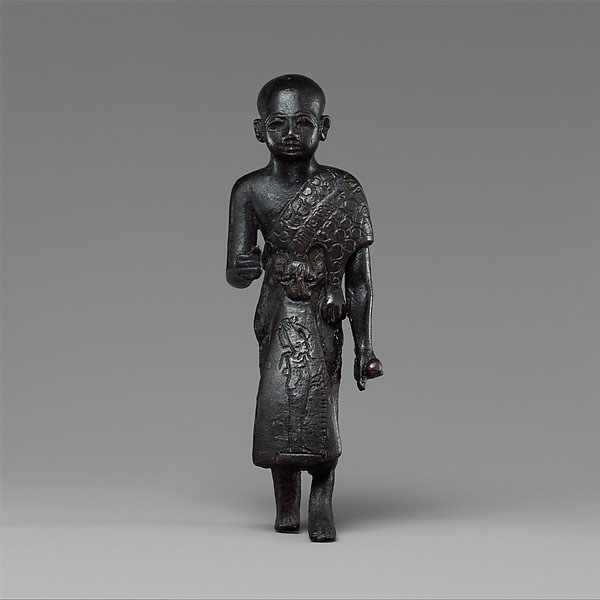
\includegraphics[width=\textwidth]{img/priest/kushite_priest}
	\caption{25th dynasty Kushite priest, with inscription of Osiris.}
\end{figure}

\subsection{Siege Tower}

\subsection{Trader (Land)}

Donkeys were the favorite travel companion for Kushite traders. They seem to have liked these rather small, hardy desert animals a lot. Long after the introduction of horses and camels, donkeys remained popular, even today. They would just pack whatever is needed on their backs, and form small, to large caravans, for long or short distance travel. The trader himself might have ridden the front donkey. Alternatively, the Beja used camels to trade back and forth with Kushite territory.

\begin{figure}[H]
	\centering
	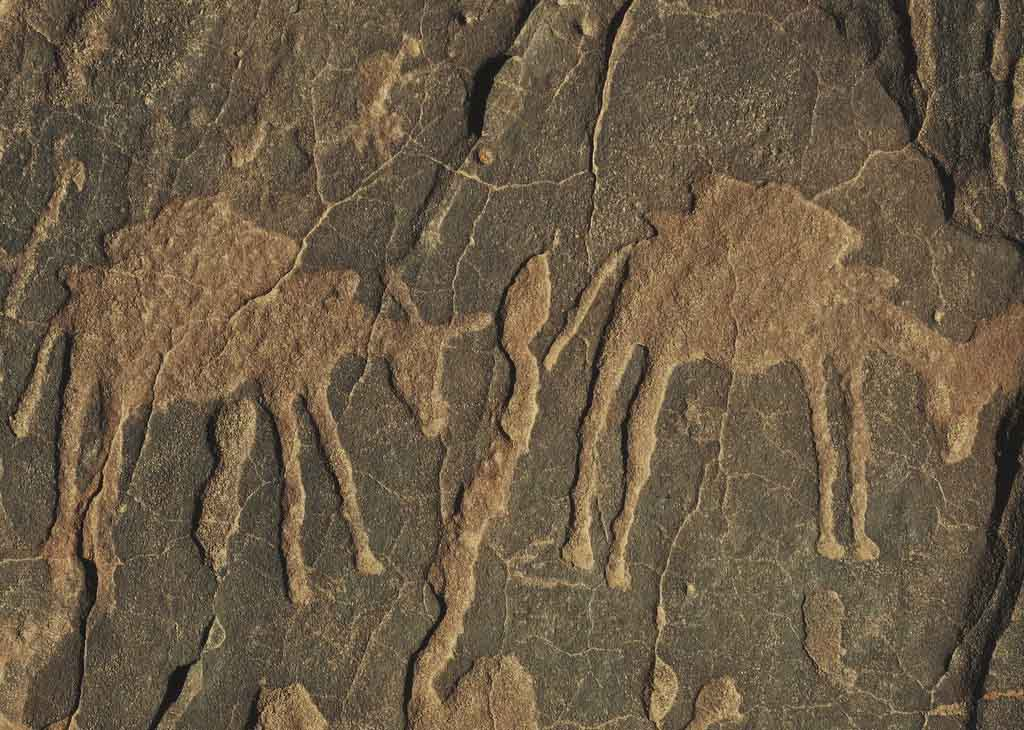
\includegraphics[width=\textwidth]{img/trader_land/petroglyphs_donkey_caravan}
	\caption{Petroglyphs in Sudan, depicting a donkey caravan}
\end{figure}

\begin{figure}[H]
	\centering
	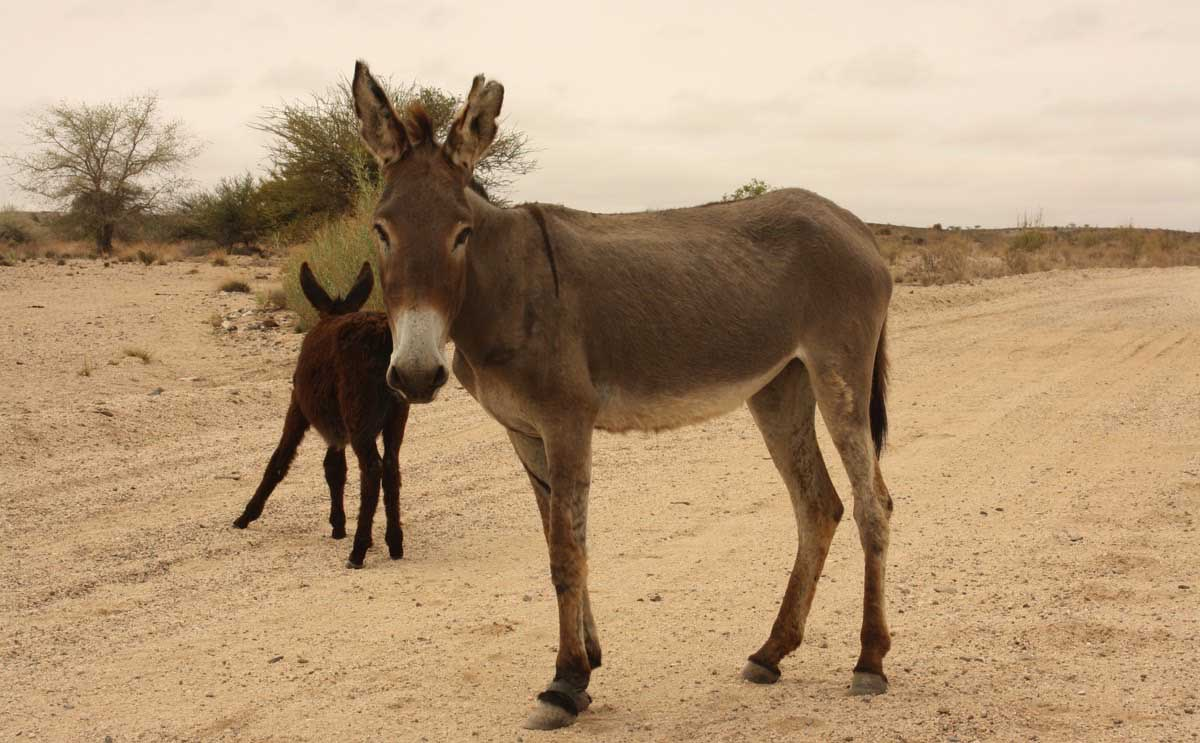
\includegraphics[width=\textwidth]{img/trader_land/donkey_sudan}
	\caption{Donkeys in Sudan}
\end{figure}

\section{Map}

Landscape: Although essentially a Nile Valley Civilization, the Kushites were not as dependent on the NIle as their northern neighbor. Many important Kushite sites are far away from the Nile, sometimes more than a 100 km away. This is largely due to the fact that the Butana steppe, the Meroitic heartland, is a seasonal savannah, as are many areas more to the south. For about 3 months in the year, the desert turns green! In Meroitic times, rainfall was markedly higher, and areas far from the Nile supported small acacia forests and large grasslands, which in turn could support larger populations than they can today.  

\begin{figure}[H]
	\centering
	\includegraphics[width=\textwidth]{img/greenery_al_azrak}
	\caption{Greenery at Al Azrak, in the border region between Sudan and South Sudan. This biotope reflects what the Kushite heartland would have looked like for several months in the year.}
\end{figure}

\section{Common Misconception}

\subsection{War Elephants}

\paragraph{Short answer:} no.

\paragraph{Explanation:}

Use of elephants for war purposes is definitely a controversial subject. Some people seem absolutely sure they had them, other seem absolutely sure they didn't. Truth is, we don't know. If they had any, they were never used to any impressive degree against either Egyptians, Persians, Ptolemies or Romans, as none of these are known to have ever actually fought against Kushite elephants. Several classical writers do mention them though. There's also a number of depictions of them, mainly in Musawwarat es Sufra, which might have been a cult place for the worship of elephants.\\

\begin{figure}[H]
	\centering
	\includegraphics[width=\textwidth]{img/slaves_and_elephant}
	\caption{Images of Elephants, wearing some kind of decorated cloth, leading a group of bound prisoners by a rope. From Musawwarat es Sufra}
\end{figure}

I actually found pictures of an elephant statuette from Meroe, dating to the Meroitic period, with a mahout and all! You'd think this closes the question, but in fact it opens up a lot more. This piece is one of a kind, and has no parallels in Nubian art. It's completely unique (so far), and doesn't seem to be of Meroitic production. But the rider does seem to carry a typical East African round shield. The features of the Mahout don't look African, perhaps even Indian. And the elephant itself actually looks Indian (two lobes on its front head). Maybe just an Indian import. Maybe a Ptolemaic import (known to use Indian Mahouts). Maybe an original Meroitic artist, depicting what he saw in Meroe. Who knows. It does seem weird to export war elephants, and not use them yourself…\\

\begin{figure}[H]
	\centering
	\includegraphics[width=\textwidth]{img/mahout_elephant}
	\caption{Elephant and mahout statuette from Meroe.}
\end{figure}

\begin{figure}[H]
	\centering
	\includegraphics[width=\textwidth]{img/mahout_two_elephants}
	\caption{Elephant statuette from Meroe. The ring on the Mahouts' head was used to suspend the piece in the air.}
\end{figure}

Another thing about the elephants, is that the African elephants used in warfare were "forrest elephants", a much smaller version of the African Bush Elephant. Bush elephants are notoriously difficult to train. The smaller size of the forrest elephants made them much easier to handle, but it also put them at a serious disadvantage against larger Indian war elephants. 

\subsection{Nubia And Related Terms}

Nubia and related terms: The term is quite confusing at times because it refers to many possible things: 1) A geographical area generally identified as the area between the 1st and the 6th cataracts. 2) Nubian people, who descend from the Noba, 4th century Nomadic settlers on the Nile between the 1st and 3d cataract. 3) Nuba people, a distinct collection of Southern Sudanic tribes, mainly in Kordofan. 4) Nubian languages, refers a Nilo-Saharan language group, spoken by the descendants of the Noba, as well as Nuba people.\\  

The Kushites pose a serious question mark here, because Kushites don't seem to be Nubian at all. They didn't speak a Nubian language, they spoke Meroitic (neither Nilo-Saharan, nor Cushitic). Nubian, in ancient Egypt, seems to refer mostly to the people directly to the south of them, and those people formed a buffer between the Egyptians and "the wretched Kush". Kushites often warred against, and subjugated the people of Lower nubia. An additional point is that Kushite territory stretched far beyond Nubia. Some of it's most important cities weren't in Nubia at all, but to the south of it. Meroe itself lies between the last two cataracts. 

\section{Weaknesses and Strengths}

All this reading has made a few things clear to me. The Kushites had particular strengths and weaknesses relevant to the game-play of 0AD.

Weakness:

\begin{itemize}
	\item Weak armor: Basic units barely used armor. Special units, champions and heroes have (quality) quilted cotton and scale armor, but they should be relatively expensive.
	\item Weak navy. Apparently no real seafaring capability (which means they’d be a weak choice for an island map). But they did have boats, and transport of troops, and basic naval defense is a definite yes. Weak boats can be compensated with garrisons of archers, firing volleys of flaming arrows (fig. 7a).
	\item Weak siege equipment: Only cursory mention of siege equipment and tactics, which include ladders, ship-masts, sapping attacks on walls, but also siege towers and battering rams.
\end{itemize}

Strength:

\begin{itemize}
	\item Infantry should have a speed bonus, because low armor makes them faster (and cheaper)

	\item Their cavalry should be particularly strong and fast. Highly desired by the Egyptians and Assyrians, the specific breed of Kushite horses was large, fast and strong. I believe it is the ancestor to the rare Dongola, or Dongolawi horse, an important breed throughout the greater Sudan in later times (disregard Wikipedia on this one. Their page dismisses the Sudanic origin of this breed, apparently based on the axiom that horses were introduced to Sudan in much later times. By now we know they were being bred by the 2nd millennium BCE, but this isn’t common knowledge I guess. In addition, the page fails to distinguish, or even identify the unique physical features of this breed. The author seems to be conflating barb and Arab horses with older African breeds).

	\item Fast chariots (drawn by two horses), shooting accurate volleys of arrows. Perfect for hit and run tactics.

	\item Large-scale food production, due to irrigation and cattle herding. Allows recruiting many, fast and cheap units early in the game, ideal for early raiding.

	\item Strong buildings and defenses. Thick walls of cut stone, dry-stone or fired brick. Mud-brick foundations provide a certain plasticity, which in turn ensures the stability of larger structures.

	\item Strong weapons. Early iron (steel) production gives them strong swords, spears and arrow tips. Maybe they should have a weak defense, but a strong attack.

	\item They were world renowned for their archery skills for several millennia. They should be the most accurate archers in the game. Even in later times, Heliodorus of Emesa mentions their “unerring skill in hitting their target, their adversaries’ eyes”. This was repeated by the invading Arabs of the Rashidun Caliphate, who called them “pupil smiters”, and were forced to retreat from Sudan with many eyes lost (battle of Dongola).  
\end{itemize}

\chapter{Art and Design}

\section{Characteristics}

\subsection{Architecture Pattern}

The temple of Apedemak \ref{fig:apedemak-temple} has a sand brown wall, which was once white in color.

\begin{figure}[H]
	\centering
	\includegraphics[width=\textwidth]{img/temple/apedemak_temple}
	\caption{A beautiful example of a temple to Apedemak, Musawwarat es Sufra}\label{fig:apedemak-temple}
\end{figure}

\subsubsection{Doors}

The Kushite doors are in the building and mostly small. Even gates in fortresses are narrow and small compared to the overall size of the building.  

\begin{figure}[H]
	\centering
	\includegraphics[width=\textwidth]{img/doors/stone_door}
	\caption{Door in a building}
\end{figure}

\begin{figure}[H]
	\centering
	\includegraphics[width=\textwidth]{img/walls_gates/qasr_ibrim_gate}
	\caption{Kushite style, narrow entrance gate to Qasr Ibrim.}
\end{figure}

\subsection{People}

Essarhadon of Assyria captured some of Taharqa's family, and described them as followed: 

\begin{center}
\textit{"His wives, his sons and [his] daughters [who]se bodies like his, have skins as black as asphalt"}\\[12pt]
\end{center}

Kush was a multi-ethnic state formed out of many tribes and kingdoms. The Meroities, the ruling class, were definitely very dark (black) in complexion. Other groups, like North Nubians and Beja were slightly lighter skinned, but still darker than the average (North) Egyptian (similar to South Egyptians though). More southern Sudanese are also very dark. The name "Sudan", means black, in Arabic, referring to its people (bilād as-sūdān, the land of the Blacks). The name Ethiopia also comes from the Greek word for Aethiopia, which means something along the line of "burnt face".

\begin{figure}[H]
	\centering
	\includegraphics[width=\textwidth]{img/people/skin_color_variances}
	\caption{ The two extremes of the ancient Sudanese phenotype (pre-Arabic). Left are modern Nubians (North Sudan and South Egypt). Notice the naturally flat hair, relatively common (but not ubiquitous) in dark skinned populations of East Africa. On the right is a modern South Sudanese man, with typically black skin (some of the darkest people in all of Africa actually). Their ancestors lived as far north as Southern Egypt in Neolithic times. They looked very similar to the Meroites. Beja also have a mix of kinky and flat hair, sometimes wearing half dreadlocks, half afro's.}
\end{figure}

Representing the Kushites with two skin-tones would be most accurate. A "lighter", reddish brown for Nubians and Beja, and a very dark complexion for Meroites and Nuba mercenaries. This would also reflect the way Egyptians represented them:    

\begin{figure}[H]
	\centering
	\includegraphics[width=\textwidth]{img/people/kushites_tribute_pharao}
	\caption{Kushites paying tribute to the pharaoh, from the tomb of the viceroy of Kush, Huy. The two skin-tones clearly represented. This image also gives a good idea of what (aristocratic) women looked like in Kush. As well as chariot design.}
\end{figure}


\begin{figure}[H]
	\centering
	\includegraphics[width=\textwidth]{img/people/kushite_gentlement}
	\caption{A perfect model of a Meroitic gentleman, ready to be armed with a variety of possible weapons. Linen or cotton cloth, wrapped around the torso provide lightweight protection from slashing weapons, and blunting other weapons. }
\end{figure}

Nuba (ethnically related to Meroites) are generally very tall and athletically built (slim to muscular).

\begin{figure}[H]
	\centering
	\includegraphics[width=\textwidth]{img/people/nuba_wrestler}
	\caption{Nuba wrestlers.}
\end{figure}

\section{Color Palette}

\begin{itemize}
	\item Buildings
	\begin{itemize}
		\item White
		\item Sand Brown
	\end{itemize}
	\item Units
\end{itemize}

\section{Textures}

\chapter{Miscellaneous}

\section{Licenses}

\begin{itemize}
	\item Code: GPL v2
	\item Documentation: GPL v2 (excluding images)
	\item Images
	\begin{itemize}
		\item External Sources: CC0 and/or CC-BY-SA 3.0
		\item Own?
	\end{itemize}
	\item 3D-Models?
	\item Sound?
\end{itemize}

\chapter{The Kingdom of Kush: A proper introduction}

\begin{center}
\textit{“Oh Great God, swift one. Who comes to him who calls. Watch my sister for me, the woman born in the same womb as me. Do for her as I have done for you. Spontaneous miracles that cannot be denied. Elevate her children and make them prosper, even as you did for me.”}\\[12pt]

\noindent
-From Taharqa’s prayer to Amun, at his temple in Kawa-
\end{center}

\begin{figure}[H]
	\centering
	\includegraphics[width=\textwidth]{img/taharqa_pharaoh}
	\caption{Taharqa, pharaoh of the 25th dynasty and father of the later Meroe period, at the temple of Amun in Napata. The holy mountain Jebel (Gebel) Barkal is in the background.}
\end{figure}

Often misunderstood, and even more often overlooked, Kush was a major center of power in the ancient world. Its deserts and its armies were the southern frontier for many classical civilizations. Its gold and ivory were prized throughout the Mediterranean and the Middle East. Its trade routes connected Africa to the rest of the world and its mercenaries served as far as Greece. It’s rulers, many of them powerful queens, known as Kandakes, ruled in the style of the Pharaohs of the New Kingdom. City builders, administrators, craftsmen and artists, ironworkers, priests, warriors, farmers, cattle herders and horse breeders. Builders of pyramids. The bowmen of Nubia. Who where these Kushites, and why would they be such an invaluable addition to 0 A.D.?

\begin{figure}[H]
	\centering
	\includegraphics[width=\textwidth]{img/meroe_pyramids}
	\caption{Some of the Iconic Nubian pyramids, at Meroe. Between the 8th Cenury BCE and 350 A.D., 255 pyramids were built by the Kushites, at El Kurru, Napata, Meroe and Nuri.}
\end{figure}

Because the Kushites have not yet been properly introduced, I will attempt to provide you with a thorough, yet concise, illustrated analysis of Kushitic history, outlining their origin and environment, culture and religion, architecture, economy and military. As well as contextualizing them in a broader Mediterranean and Middle Eastern world, around the time frame of 0 A.D., including the prolonged wars they waged against several civilizations already featured in the game. Because of the lack of credible and historically accurate representations of these people in popular culture, I have spent some time, gathering a rich collection of historically accurate and relevant images, focused on important archaeological sites, and accurate reconstructions of houses, monuments, cities and the people and attire of various classes and backgrounds within Kush. If any attempt is made to represent “The Kingdom of Kush” in 0 A.D., the images provided in this introduction can provide the backbone for models of buildings and units, as they represent some of the most historically accurate images available on this civilization.

\begin{figure}[H]
	\centering
	\includegraphics[width=\textwidth]{img/king_tanyidamani_and_apedemak}
	\caption{King Tanyidamani and Apedemak, the god of war and fertility, on a votive plaque from the Naqa kiosk.}
\end{figure}

\section{Indentifying Kush}

Kushites are known and referred to by a number of names, sometimes confusing the casual reader trying to find out more about these people. The following names are used interchangeably: “Kush”, or “The kingdom of Kush”, “The Kushitic empire”, “Napatans”, “Meroites”, “The Meroitic Empire” or more commonly, but less precisely, “Nubia”, or “the Nubians”. Egypt’s fearsome southern neighbor. This is Herodotus’ Aethiopia (Ethiopia). It must not be confused with the modern day country of Ethiopia, which lies to the south of ancient Kush. Neither should they be confused with the “Kushans” of Bactria and India. The Kingdom of Kush was centered in modern day Sudan. More specifically on the Butana step, a vast, semi-arid, seasonal savannah, flanked by the Nile and the Blue Nile to the West, and the Atbarah River to the East. There, people took advantage of seasonal rainfalls to engage in large-scale agro-pastoralism. Mainly cattle herding and the cultivation of barley, wheat, sorghum and millet, along with cash crops like cotton and dates. In 450BCE Herodotus correctly identified the capital as Meroe, an ancient site that was used for royal burials as early as 890BCE. Situated between the 5th and the 6th cataract on the Nile, Herodotus called it a “great city... said to be the capital of the other Ethiopians”.

\begin{figure}[H]
	\centering
	\includegraphics[width=\textwidth]{img/map_of_kush}
	\caption{A map of Lower, Upper and South Nubia, in modern day Sudan. The core of Kushite influence stretched about a thousand km, from the first cataract around Maharraqa (traditionally the Roman frontier), to Jebel Moya.}
\end{figure}

\section{Early History: Kerma and Napata}

\textbf{(Before the time frame of 0 A.D.) c. 3500BCE - 590BCE}\\

The Kingdom of Kerma is the first expression of Kushite culture. The Pre-Kerma period, beginning around 3500BCE, saw the development of the earliest known, dense settlement patterns in Sub Saharan Africa. By 2500BCE Kerma emerged as a regional center, and by 1700BCE the city of Kerma had an estimated population of over 10.000 people. It boasted monumental buildings and a system of thick defensive walls, miles of irrigation canals and engaged in long distance trade. It was the seat of a centralized state. The first of many in Sudan. 
 
\begin{figure}[H]
	\centering
	\includegraphics[width=\textwidth]{img/central_kerma}
	\caption{A view of central Kerma around 2000BCE. The large structure in the center of the town, presumably a temple, is called The Western Deffufa. It's impressive ruins still stand today. This image is based on the archaeological surveys revealing the town plan in relative detail.}
\end{figure}

The Kingdom of Kerma is attested in Egyptian records as Kush (k3š), as early as the Middle Kingdom, and its riches had been prized since the Old Kingdom. Then, starting with Senusret I, and particularly Senusret III of 12th Dynasty, Egypt gained its first permanent foothold in Lower (northern) Nubia, with the establishment of massive forts, such as Buhen in c. 1860BCE. By the 13th dynasty, Egyptian power waned, the forts were abandoned and Lower Nubia was reoccupied by Kush. By c. 1550BCE Kerma was strong enough to challenge Egypt itself, formed an alliance with the invading Hyksos from the north, and raided deep into Upper Egypt. These events almost brought about a premature end to Pharaonic Egypt, and led to the Second Intermediate Period. Curiously, Nubian bowmen served as mercenaries (the original Medjay), in Kamose’s campaign against their former Hyksos allies. 

\begin{figure}[H]
	\centering
	\includegraphics[width=\textwidth]{img/pharaoh_kamose_battle_plan}
	\caption{Pharaoh Kamose revealing the battle plan to his Kushite allies, during his "war of liberation" against the Hyksos.}
\end{figure}

Under Kamose, and the subsequent reestablishment of Egypt under the New Kingdom with Amenhotep I and Thutmose I, Kush was invaded several times, and Kerma was destroyed. For the next 500 years, upper and lower Nubia effectively became increasingly Egyptianised colonies, though the relationship was often of a symbiotic nature. 

\begin{figure}[H]
	\centering
	\includegraphics[width=\textwidth]{img/new_kingdom_battle}
	\caption{A New Kingdom Pharaoh campaigning in Lower Nubia.}
\end{figure}

In the 15th century BCE, Thutmose III established a small temple in Nubia at the foot of Jebel Barkal, a modest, lonely mountain rising steeply from the flat desert floor surrounding it. It was said to be the southern home of Amun, and marked Egypt’s southern most expansion. The existing town, now called Napata, was to become one of the most important centers of Kush. As it’s religious capital, it became the seat of the cult of Amun. Around 1075BCE, the New Kingdom collapsed, and the Egyptianised people of Kush set up an independent kingdom, centered on Napata. This ushered in the Napatan period.\\

By 721 BCE, the Napatans had become so powerful, that their king, Kashta, invaded Upper Egypt and occupied Thebes. His successor, Piye, completed the conquest, and conquered one of the largest empires the Nile Valley had ever seen. Piye, Shabaka, Shebitku, Taharqa and Tantamani all ruled Egypt, as well as Kush, as pharaohs of the 25th dynasty, also known as the “Nubian Dynasty” or the “Kushitic Empire”. They saw themselves as the custodians of Egyptian culture and religion. Piye built the first pyramid the Nile Valley had seen in over 500 years, a tradition the Kushite kings continued in to the 4th century A.D. They initiated major restoration projects on the ancient temples, and built many new ones, reinvigorating Egyptian traditional religion (especially the cult of Amun), as well as collecting tribute from powerful states in the Levant and expanding their military activity as far north as Judea.   

\begin{figure}[H]
	\centering
	\includegraphics[width=\textwidth]{img/piye_troops_take_memphis}
	\caption{Piye's troops take Memphis, the northern capital, thereby unifying all of Egypt and all of Kush.}
\end{figure}

\begin{figure}[H]
	\centering
	\includegraphics[width=\textwidth]{img/piye_tribute}
	\caption{The Pharaoh Piye receiving tribute from Egyptian royals.}
\end{figure}

Growing tensions over Kushite activity in the Levant, led to a series of devastating wars with the Neo-Assyrian Empire beginning in 677BCE. In 671BCE, Taharqa fought running battles with the armies of Esarhaddon from the Sinai to Memphis, but was defeated, and fled to Thebes. Taharqa’s wife (and/or sister) and son, were both captured and taken to Nineveh. Tantamani restored Kushite rule in Egypt to some extent, but by 656BCE, Psamtik I of the Saite Dynasty took control of Thebes, ending the Kushite presence in all of Egypt. Psamtik II, with the participation of Greek mercenaries, campaigned in Lower Nubia. By 590BCE the Kushite seat of authority was shifting towards the more southern Meroe, eclipsing Napata, and giving rise to a distinctively more “Africanised” Meroitic culture. The Neo-Assyrian Empire collapsed in 609BCE, and was absorbed by the Persian Achaemenid Empire under Cyrus the Great. His successor, Cambyses II, successfully conquered Egypt in 525BCE, after which he attempted the conquest of Kush. He was met with catastrophic failure, possibly because of the difficulties associated with marching an army through the desert.

\begin{figure}[H]
	\centering
	\includegraphics[width=\textwidth]{img/assyrian_vs_nubian}
	\caption{An Assyrian and a Nubian fight it out, in one of many battles fought during the Assyrian invasion of the Levant and Egypt.}
\end{figure}

By all accounts, the Pharaohs of the 25th dynasty, especially Piye and Taharqa, are to be considered the fathers of the later Meroitic period, and its subsequent rulers. The Kings of Meroe went to great lengths to preserve the Egyptiansed customs they inherited. But neither did they shy away from developing their own, independent culture, religious practices, writing systems, architectural styles, aesthetic principles, military systems and trade networks. They also incorporated Greco-Roman, Ptolemaic, Persian and Indian influences. Combined with their close proximity to very warlike, sometimes nomadic, African tribes (like the Blemmyes) and the assimilation of many of these tribes in to a greater Kushite state, demonstrate a level of social complexity rarely seen in this region in later times. The complex interaction of many peoples, cultures and influences, increasingly transformed Meroe in to a uniquely African civilization. It is this later expression of Kushite culture, during the Meroitic period that we shall examine further. Starting around 590BCE, when Meroe started eclipsing Napata, and ending with the Axumite invasions of Kush, around the 330's AD, the Meroitic period spans the entire length of 0 A.D.’s timeframe and beyond.

\begin{figure}[H]
	\centering
	\includegraphics[width=\textwidth]{img/naptan_kings}
	\caption{In a pit, close to Kerma, the broken statues of a number of Napatan Kings were uncovered, including some of the 25th dynasty, and later Kings. The known kings are: Taharqa, Tanoutamon, Senkamanisken, Anlamani and Aspelta. This find, along with others, show that Kerma was still important, long after its destruction, and it also shows a clear continuity from the 25th dynasty to later Kushite kings.}
\end{figure}

\section{The Meroe Period}

\textbf{(During the time frame of 0 A.D.) c. 590BCE – 330AD}\\

Napata was essentially a southern expression of classical Egyptian culture. In fact, it can be said that during the height of the Napatan 25th dynasty, the material culture of Nubia and Egypt become indistinguishable. The same cannot be said for Meroe. The move to Meroe symbolizes a break from the strict, Egyptian character of the earlier Napatan Period, and saw the mixing of African, Egyptian, Middle Eastern and Mediterranean influences. Napata remained one of the most important cities in Kush, though, and the Kings of Meroe built new temples and palaces, maintaining its religious authority throughout the Meroitic period.

\begin{figure}[H]
	\centering
	\includegraphics[width=\textwidth]{img/napta_temple_district}
	\caption{Detailed plan of excavation results in Napata, showing the central "temple district", with many temples to various gods and even 2 visible palaces.}
\end{figure}

\begin{figure}[H]
	\centering
	\includegraphics[width=\textwidth]{img/holy_mountain_jebel_barkal}
	\caption{Napata in it's full glory around the 1st century BCE, infront of the holy mountain, Jebel Barkal. King after King commissioned restorations and new temples. Even after the move to Meroe, many kings continued to be crowned here. This illustration stays true to archaeological reports on the site.}
\end{figure}

Possibly prompted by increasing hostility from Egypt and the Persians to the north, the more southern Meroe became increasingly important. Another possible reason for the move south, is that the Napatan Kings of Kush were trying to brake from the authority of the cult of Amun, the foremost religious authority in Kush, also centered in Napata. By moving the royal capital to Meroe, the society was secularized, and the Kings enjoyed a greater freedom than before. This move was completed by the time of Arakamani, identified with “Ergamenes”, of Diodorus Siculus’ Bibliotheca Historica, in the early third century BCE. According to Diodorus, the priesthood of Amun had the power to order the death of a king. Ergamenes (Arakamani), was the first King to brake from this tradition, when the priests ordered his death. He moved on Napata, ordered the massacre of the priests, and moved the royal burial grounds to Meroe, where many of the iconic Meroitic pyramids were built. Diodorus states that his strong will came from his instruction in Greek philosophy, probably related to the rule of the Ptolemies in Egypt. Regardless of the changing relationship between the kings and the cult of Amun, the worship of Amun remained important throughout Kushite history. Temples to Amun continued to be built in to the third century A.D., and the cult was still present during the Christianization of Nubia in the 6th century A.D. 

\begin{figure}[H]
	\centering
	\includegraphics[width=\textwidth]{img/temple_of_amun}
	\caption{Remains of the temple to Amun, in Naqa. Built by Natakamani in the 1st century A.D.}
\end{figure}

\begin{figure}[H]
	\centering
	\includegraphics[width=\textwidth]{img/remains_colonnade_naqa}
	\caption{The Remains of a colonnade in Naqa, depicting the god Bes.}
\end{figure}

\begin{figure}[H]
	\centering
	\includegraphics[width=\textwidth]{img/kandake_religious_procession}
	\caption{A Kandake leading a religious procession in one of the temples in Napata}
\end{figure}

With the move to Meroe, a local South Nubian deity, known as Apedemak, rose to prominence. This lion headed god of war might have even eclipsed the worship of Amun. During the Meroitic period, many new temples were built, in Napata, Naqa, Wad Ben Naqa, Musawwarat es Sufra, Hamadab, Dangeil and other important centers. Usually to Amun or Apedemak, but also to Hathor and Isis, and some temples and shrines were also dedicated to lesser-known Nubian gods. Although stylistically still Egyptian, the floor plan of these temples was typically Kushite.

\begin{figure}[H]
	\centering
	\includegraphics[width=\textwidth]{img/temple/apedemak_temple_profile}
	\caption{Temple to Apedemak, the lion headed god of war, in Musawwarat es Sufra}
\end{figure}

\begin{figure}[H]
	\centering
	\includegraphics[width=\textwidth]{img/temple/apedemak_temple}
	\caption{A beautiful example of a temple to Apedemak, Musawwarat es Sufra}
\end{figure}

The Meriotic period also saw the infiltration of Indian and Persian influences (in depictions of deities, imported textiles), Greco Roman (in the form of luxery imports, stylistic additions to temples and monuments, or the Roman bath-house in the Royal City in Meroe and lavish Mediterranean style decorations in elite residences) and Ptolemaic (in the form of Greek philosophy, military technology and import of luxery goods, like wine). The Meroitic period also saw the embracement of typically Sub Saharan African ethno-cultural elements. They still, more or less, depict themselves in Egyptian styles, but with typically black African physical features. Intense contact with often hostile and nomadic or semi-nomadic desert tribes, as well as other more southern tribes, and their subjugation to Kushite rule and incorporation in to the state, was necessary to keep trade routes open. Trade routes like those connecting Meroe to the Mediterranean, and the Red Sea coast (Eritrean Sea), where it was connected to the Indian Ocean trade. Meroe slowly grew in to a metropolis.

\begin{figure}[H]
	\centering
	\includegraphics[width=\textwidth]{img/plan_excavated_structures_meroe}
	\caption{A plan of the main excavated structures in Meroe, including the "Royal City", temples to Amun, Apedemak and Isis, as well as other shrines. The large heaps in between the temples in front of the Royal City are city mounds. The remains of sprawling residential areas.}
\end{figure}

\begin{figure}[H]
	\centering
	\includegraphics[width=\textwidth]{img/13b_Reconstruction_of_Meroe_from_The_Capital_of_Kush_by_Rebecca_J_Bradley}
	\caption{A historical reconstruction of the city of Meroe, around 100 A.D. From "The Capital of Kush" by Rebecca J Bradley.}
\end{figure}

\begin{figure}[H]
	\centering
	\includegraphics[width=\textwidth]{img/roman_kiosk}
	\caption{The Naqa kiosk, aptly nicknamed the Roman Kiosk, because of its Greco-Roman features. Corinthian capitols and Roman, stone cut arched windows attest to the far flung influence in this structure.}
\end{figure}

The Meroe period saw a number of interesting indigenous developments, such as the “Nubian vault” and smaller domes. Palaces as well as common residential buildings were often constructed with vaulted ceilings made of brick. This was especially useful in an arid climate were trees aren’t large or plentiful enough to provide roofing material. Large, multistoried square palaces, built over vaulted cellars became common. Thick walls and small (arched) windows on the ground floor of these palaces hint at a secondary defensive purpose.

\begin{figure}[H]
	\centering
	\includegraphics[width=\textwidth]{img/civic_center/governor_palace_karanog}
	\caption{A small governors' palace in Karanog, lower Nubia. This building features typical Nubian architecture, with vaulted ceilings, open courtyard and square design. Small windows and thick walls on the lower floor hint at a defensive purpose. A lavishly decorated 2nd floor served as the living space for the governor and his family "Fabricated by Christ Ray, in collaboration with David O'Connor and Stacey Olson, from plans an descriptions of the 1907 excavation"}
\end{figure}

Regular houses were often compound structures, made up of rectangular blocks, arranged around private courtyards. Either using vaulted ceilings, or flat plastered roofs, supported by thick palm logs, making use of columns for extra support. Extra floors were added for expansion, as families grew, and flat roofs often had stairways leading up to them. Houses were built with sundried mud brick, or fired red bricks. Wealthy households and official buildings made use of cut stone for doorways and windows. Usually these brick buildings received a cover of fine white, lime plastering, creating a smooth white surface, sometimes decorated with colored, geometric motives, or religious symbols, especially around the doors and windows. An important note is that contemporary Nubian homes and settlement patterns, around Aswan and North Sudan, are strikingly similar to those of the Meroitic period, and even the earlier Kerma period.

\begin{figure}[H]
	\centering
	\includegraphics[width=\textwidth]{img/house/meroitic_double_house_floor_plan}
	\caption{Floor plan of a Meroitic double house in Al-Meragh. Two identical halves, but completely separated from each other by a thick dividing wall. This was only one of a number of nearly identical structures in the immediate area.}
\end{figure}

\begin{figure}[H]
	\centering
	\includegraphics[width=\textwidth]{img/house/3d_model_of_meroitic_double_house}
	\caption{3d rendered model of the Meroitic double house at Al-Meragh. Built with brick, it's doorways were lined with cut stone. The outside of the house received a fine white lime plastering. Stairs leading up to a flat roof, probably used for a variety of purposes.}
\end{figure}

\begin{figure}[H]
	\centering
	\includegraphics[width=\textwidth]{img/house/double_house_inside}
	\caption{Inside the central living room in one half of the Al-Meragh compound. Stone pillars and capitols support wood beamed roof. Small windows allow for light and air circulation, but they are small enough to keep out unwanted guests.}
\end{figure}

\begin{figure}[H]
	\centering
	\includegraphics[width=\textwidth]{img/house/nubian_vault_sketch}
	\caption{A modern example of an ancient design. Featuring the Nubian vault and arched windows. Many common houses in Meroitic Kush would have looked identical to this one.}
\end{figure}

\begin{figure}[H]
	\centering
	\includegraphics[width=\textwidth]{img/house/recreation_nubian_architecture}
	\caption{A recreation of a meroitic house in the Nubian Museum in Aswan. Rectangular rooms, with vaulted ceilings arranged around a central courtyard. Mud plaster and painted decorations finish the design.}
\end{figure}

Iron appears in Meroitic sites from 600 BCE. Huge mounds of iron slag, associated with near-industrial levels of iron production in the Meroe area, dating from both the Meriotic as well as the post Meriotic period, attest to the importance of this new metal. Because of it, Meroe has been dubbed “the Birmingham of Africa”.

\begin{figure}[H]
	\centering
	\includegraphics[width=\textwidth]{img/iron_smelting}
	\caption{Iron Smelting in Meroe}
\end{figure}

\begin{figure}[H]
	\centering
	\includegraphics[width=\textwidth]{img/iron_working_drawing}
	\caption{Iron working in Meroe, to create tools and weapons.}
\end{figure}

\begin{figure}[H]
	\centering
	\includegraphics[width=\textwidth]{img/iron_slag_excavated}
	\caption{Large mounds of Iron slag around Meroe being excavated.}
\end{figure}

\begin{figure}[H]
	\centering
	\includegraphics[width=\textwidth]{img/iron_weapons_and_tools}
	\caption{Iron weapons and tools from Meroe.}
\end{figure}

Meroe grew in to a center of production and trade. A military power, that campaigned as far south as the Sud, and the borders of modern day Ethiopia. Against the desert tribes to the East and West of them, and against their Northern neighbor, Egypt, whether Egypt was under Native, Persian, Ptolemaic or Roman rule. It wasn’t until the shifting of trade routes, and increased activity of desert tribes, that Meroe started waning in importance. The straw that finally broke the camels back, were the Axumite invasions of the 330’s A.D. 

\section{Something on the written record}

Meroitic script was developed, and replaced Egyptian writing systems to a large extent, by the third century BCE. Meroitic script still hasn’t been deciphered, and this limits what we know about the internal workings of the Kushite state, or their precise relation to outside powers, in the Meroe period. For example, what was the importance of horses in Kushite society? Luckily we have other sources to our disposal, which give us valuable insights.

\begin{figure}[H]
	\centering
	\includegraphics[width=\textwidth]{img/merodic_script}
	\caption{A beautiful example of Meroitic script}
\end{figure}

An example is Piye’s victory stele in Napata, written in Egyptian hieroglyphs. Here he expresses outrage at the sight of neglected horses in the stables of the newly conquered Hermopolis:\\

\begin{center}
\textit{"I swear, as Re loves me, and as my nostrils are rejuvenated with life, it is more grievous in my heart that my horses have suffered hunger, than any evil deed that thou hast done, in the prosecution of thy desire."}\\[12pt]
\end{center}

The text also notes the frequent use of horses and chariots in his campaigns, and that they are paid to him as tribute. Other examples are the Neo Assyrian palace records under Sargon II, Esarhaddon and other rulers, which make frequent mention of “Kushite horses”, “Kushite riders” “Kushite horse trappings” and “Kushite charioteers” and chariots. Kushite horses and chariots were captured during the Assyrian invasions of Egypt, and Kushite horses were a prized trade commodity in earlier as well as later times. The large, Kushite breed of horse apparently being much desired, was exported on a considerable scale, along with their handlers and charioteers. These records, along with the finds of horse remains in the tombs of some kings, clearly show that horses were bred, and played an important role in Kush, as they did in later periods of Sudan’s history.

\begin{figure}[H]
	\centering
	\includegraphics[width=\textwidth]{img/horses_tribute}
	\caption{Horses as tribute to King Piye, Napata}
\end{figure}

In the 4th century BCE, the Kushite King Nastasen erected a victory stele, written in hieroglyphs, boasting of a victory against an invasion from Egypt, led by Kambasuten. Nastasen claimed to have taken “many fine boats”. Kambasuten is widely identified with Khabash from Sais, who lead a revolt against Persian rule in Egypt, just a few years before the conquest of Alexander the Great.

\begin{figure}[H]
	\centering
	\includegraphics[width=\textwidth]{img/king_nastasen_stele}
	\caption{King Nastasen's victory stele}
\end{figure}

In other, foreign records, such as “On the Erythraean Sea”, Agatharcides states that Ptolemy II equipped 100 cavalrymen with “Kushite style quilted armor”, for his Nubian campaign in the 270’s BCE. This Nubian campaign resulted in an uneasy occupation of the Dodecaschoenus, a 75-mile strip of land south of the 1st cataract, resulted in decades of fighting and ended with the Nubian reconquest in the 210’s, followed by Kushite-supported revolts in Upper Egypt. Agatharcides’ text also indicates that Kushites had been using quilted (cotton?) armor since at least the third century BCE. This typically Sudanic quilted armor, often used by cavalry and particularly useful against poisoned arrows, became ubiquitous to the greater region up until modern times.
 
\begin{figure}[H]
	\centering
	\includegraphics[width=\textwidth]{img/king_tanyidamani_armor_soldier}
	\caption{The soldier on the right is from the kingdom of Makuria, post-Meroitic period. He's wearing quilted armor, which I believe is what King Tanyidamani (c. 100 BCE) is wearing, pictured on the left votive plaque. I'm strengthened in this idea, because he is wearing the Hemhem crown, associated with battle, and the reverse of this votive features Apedemak, god of war, in scale armor, indicating a military context. Minus the shield and helmet, replaced with a more fitting helmet and shield, the soldier on the right would be a good medium infantry unit.}
\end{figure}

One of the most interesting events of this period was recorded by Strabo, in his “Geography”, and relates the invasion of Upper Egypt by Queen Amanirenas and her son, Akinidad in 27BCE, which started a 5-year war with the Romans. Strabo goes on to say:\\

\begin{center}
\textit{“…The Ethiopians, emboldened in consequence of a part of the forces in Egypt being drawn off by Aelius Gallus, who engaged in war with the Arabs, invaded the Thebaïs and attacked the garrison, consisting of three cohorts, near Syene; surprised and took Syene, Elephantine, and Philae, a sudden inroad; enslaved the inhabitants, and threw down statues of Caesar. But Petronius, marching with less than 10,000 infantry and 800 horse against an army of 30,000 men, compelled them to retreat to Pselchis, an Ethiopian city. He then sent deputies to demand restitution of what they had taken, and the reasons which had induced them to begin the war…”}\\[12pt]
\end{center}

\begin{figure}[H]
	\centering
	\includegraphics[width=\textwidth]{img/heros/queen_amanirenas_roman_fort_burn}
	\caption{Queen Amanirenas and her son Akinidad watch a Roman fort burn to the ground, in 27 BCE, during their invasion of Upper Egypt. The inspiration for the attire of the royals being depicted was taken directly from the reliefs in various temples}
\end{figure}

After 3 days of silence from the Kushites, the Romans attacked, defeated Amanirenas and pushed deep in to Kushite territory until they reached Napata. They razed the city, after which they retreated back to Premnis. The war ended with a negotiated peace treaty, remarkably favorable to the Kushites. The Romans even ceded Premnis, in return for the many statues the Kushites had looted. An interesting side-note, is that the head of one of these statues, a bronze head of Emperor Augustus (known as the Meroe Head), was buried beneath the steps of a temple of victory in Meroe, as if to insult the Roman Emperor. It was excavated by J. Garstang in 1910, and is now on display in the British museum.

\begin{figure}[H]
	\centering
	\includegraphics[width=\textwidth]{img/augustus_bronze_head}
	\caption{The Bronze head of Augusts, known as the Meroe head, found buried beneath the steps of a temple to victory in Meroe.}
\end{figure}

The Noba, formerly a nomadic tribe wondering the Western Desert, became a Roman foederati in the north in 297 A.D (Nobatae), and a Kushite vassal in the south. The aggression of these Noba became an increasing liability to the Kushite state, eroding central authority. By the 330’s AD, the Axumite Empire, centered in modern day Ethiopia and Eritrea, had become strong enough to challenge a weakening Kush, and the Axumite Emperors Ousanas, and his successor, Ezana, waged wars against Kush. Although Ezana’s campaign seems to have been directed primarily against the Noba, in response to Kush’s inability to deal with their raiding activities on the Sudan/Ethiopia border. Ousana’s and Ezana’s invasions laid waste to Noba, and Kushite territory, effectively ending Kushite hegemony. Ezana commemorated his victory on a stone tablet, called the “Ezana Stone”, written in Ge’ez, Greek and Sabaean. A part of its translation reads:\\

\begin{center}
\textit{ 13.Then, when I had sent them [further] messages they did not heed me, and they refused to desist and […]. 14.But they retreated once I made war on them and I rose up by the power of God 15.and killed [them] by the Takkazē at the ford of Kemalke while they took to flight 16.without making a stand. And I pursued the fugitives for twenty-three days, kil17.ling them, taking prisoners, and seizing booty wherever I halted, while 18.my troops who had gone forth into the surrounding country brought back [further] prisoners [and] booty and I burned their towns 19.of brick and those of straw. And they (i.e., the Aksumite troops) pillaged their grain and copper and iron and 20.[…..] and destroyed the idols in their temples and the storehouses of grain and cotton and cast 21.them into the Nile. And many—I know not their number—died in the water 22.as their boats sank from being overloaded with people, 23.women and men.}\\[12pt]
\end{center}

\begin{figure}[H]
	\centering
	\includegraphics[width=\textwidth]{img/trilingual_ezana_stone}
	\caption{The trilingual "Ezana Stone", in Axum, Ethiopia, detailing Emperor Ezana's campaign against Kush. Ezana is noted for being the first Christian ruler of Axum.}
\end{figure}

These kind of written records, combined with a relative wealth of archaeological records and an understanding of the pre-Meroe period as well as the post Meroe period, allow us to piece together a relatively coherent, and accurate narrative of the Kingdom of Kush during 0 A.D.’s timeframe.\\

Of all the records, the archaeological record is probably the most telling. The remains of planned, and sometimes walled and fortified cities, temple complexes, royal palaces, worksites, statues and pyramids, associated with hieroglyphs and meroitic script, funerary gifts, ancient graffiti and religious depictions, give us something very tangible. Something that we can use to bring this great, forgotten civilization back to life.

\begin{figure}[H]
	\centering
	\includegraphics[width=\textwidth]{img/map_of_ancient_hamadab}
	\caption{Using ground penetrating radar to examine sub surface remains, a detailed map of ancient Hamadab became visible. A walled Meroitic town, 3km south of Meroe. There was an administrative center, temple, worksites for the production of pottery and iron manufacturing.}
\end{figure}

\begin{figure}[H]
	\centering
	\includegraphics[width=\textwidth]{img/3d_visualization_hamadab}
	\caption{3d visualisation of the town plan of Hamadab}
\end{figure}

\begin{figure}[H]
	\centering
	\includegraphics[width=\textwidth]{img/rendering_hamadab}
	\caption{A final rendering. A preliminary idea of what the town of Hamadab looked like.}
\end{figure}

\section{Something on weapons and armor}

We don’t know a lot about the Meroitic military, but we know some things. Apart from the typical shield and spear, daggers and massed archery, new weapons and tactics were being introduced. Swords, mounted cavalry, armed with lances, cavalry archers, leather armor, as well as quilted armor and the introduction of Hellenized helmets (and possibly armor) for some infantry and cavalry, probably explained by their mercenary activities in Ptolemaic Egypt. For the most part though, it seems that Nubian forces were poorly armored. Nubian archery remained important into Islamic times. New types of clothing became common. Kings were now seen wearing capes, thick jackets covering their arms, and wore simple belts decorated at the tips. By the beginning of the post-Meroitic period, 4th century AD, chain mail is attested, and scale armor was used by (royal?) elites since the New Kingdom. Large oblong shields of ox-hide were used by the Meroites, as well as smaller, round elephant- hyppo- or rhinoceros-hide shields. Beja (also known as Blemmyes), a Kushite enemy, vassal at times, and eventual overlord (Beja dynasty), used distinct east African round shields of this hardened leather type. Beja used mounted camel units, to dominate the deserts East of the Kushite heartland, from where they frequently raided Roman territories in Upper Egypt, making use of imposing swords, lances and sometimes thick ox-leather armor. They are perfect mercenary units for the Kushites.\\

 Besides these fragmentary bits of information on weapons and armor in the Meriotic period, we can assume that the Kushites inherited many New Kingdom Egyptian military elements. As the 25th dynasty had full access to the Egyptian military, this conclusion seems logical and this is attested by the production, use and export of Egyptian chariots as early as the New Kingdom, well in to the Napatan period. The New Testament story of Phillip and the (“Ethiopian”) Eunich, suggests that chariots were still used past the turn of the millennium. Kushite kings are often depicted wearing Egyptian style armor and weapons in addition to native swords. There is controversy about the use of war elephants in Meroe. It has been mentioned in a number of classical texts, but hard evidence is lacking. We only have a handful of depictions of elephants in ancient Meroe, from which we can only deduce that elephants were tamed. They were worshipped to some extent (Musawwarat es Sufra), and their use might have well been limited to ceremonial purposes like parades. Other, older weapons were still used, like battle-axes, stone maces and even clubs, some of which were inlaid with sharp stones, remarkably similar to the Aztec Macuahuitl.\\
 
\begin{figure}[H]
	\centering
	\includegraphics[width=0.8\textwidth]{img/king_tarekeniwal_slays_enemies}
	\caption{King Tarekeniwal, about to brutally slay his enemies with some type of battle axe. His entire body including his arms and upper legs are covered in scale armor, and he's wearing a typically Egyptian skull cap with chinstrap.}
\end{figure}

\begin{figure}[H]
	\centering
	\includegraphics[width=\textwidth]{img/heros/prince_arikankharer_slays_enemies}
	\caption{Prince Arikankharer slaying his enemies with a battle axe, while holding on to a sword. A second sword, tucked in his belt, is still in it's scabbard.}
\end{figure}

\begin{figure}[H]
	\centering
	\includegraphics[width=\textwidth]{img/nubien_bowmen/nubien_bowmen}
	\caption{The classical Nubian Bowmen we're all too familiar with. On the right, we see a typical Nubian chief.}
\end{figure}

\begin{figure}[H]
	\centering
	\includegraphics[width=\textwidth]{img/life_kush_drawing}
	\caption{Angus McBride does not disappoint us, with this sumptuous depiction of life in Kush. Note the "tribal warrior's" shield is made of tightly woven wicker. The Meroitic warrior, apart from his short sword and bow and arrow, is wearing a typically Nubian thumb ring, to protect his thumb during archery. The Meroitic lady sits with uncovered bosom, as they were sometimes depicted. }
\end{figure}

\begin{figure}[H]
	\centering
	\includegraphics[width=0.6\textwidth]{img/ptolemaic_egypt_mercenary}
	\caption{Nubian mercenary cavalry from Ptolemaic Egypt. Wearing pants, a Phrygian cap, and possibly Hellenistic armor, as well as a double axe. Although this unit isn't Merioitic, such mercenary units would have brought back new weapons, technology and ideas upon their return to Nubia.}
\end{figure}

\begin{figure}[H]
	\centering
	\includegraphics[width=\textwidth]{img/kushite_cavalry/meroitic_cavalry_man}
	\caption{This Meroitic cavalry man is wearing a helmet with chinstrap, possibly some kind of variation of the Boeotian helmet.}
\end{figure}

\begin{figure}[H]
	\centering
	\includegraphics[width=\textwidth]{img/kushite_cavalry/sketch_meroitic_cavalry_man}
	\caption{1st Century BC Meroitic cavalry man, with a lance, tight fitting skullcap, wearing a cape, and mounted on a horse with at least some minimal decoration. He might also be wearing pants and slippers. traced from a relief in temple "Meroe 250".}
\end{figure}

\section{Some notes and my Conclusion}

By now, you will have undoubtedly realized the potential for the Kingdom of Kush as an exciting new faction in 0 A.D. I just want to remark on the similarities between ancient Egypt, the Ptolemies and the Kingdom of Kush.\\ 

It is easy to fall for the narrative of Nubia as an Egyptian backwater due to the near obsession with Egyptian studies, which have overshadowed the more modest Nubiology. But the archaeological record is slowly being reexamined, old and new sites are being excavated and new discoveries are being made. Previous preconceptions are being questioned, and wholly abandoned in some cases. Especially the nature of the relationship with Egypt.\\ 

Much of the architectural identity of Kush, is clearly a native development, with the notable exception of Temples, which have a clear New Kingdom influence. That having said, even the temples are unique in terms of their floor-plan, the gods worshipped there, and their stylistic influences. Settlement patterns remain relatively consistent throughout the history of Kush, since predynastic times. Common structures show clear continuity with Kerma culture, and feature unique developments, like vaults, open courtyards, arched windows and Nubian decorations. Palatial structures and administrative centers are also uniquely Nubian. They were monumental, multistoried structures, built with brick and stone, according to strict, square floor plans (sometimes exceeding 60m x 60m), around a central, enclosed courtyard, illuminated by a light well. White lime plaster and brightly colored colonnades were popular, and stone and brick columns were common in general. Thick defensive walls were built around important settlements, featuring cut stone foundations, and fired brick constituting the upper layers. Bastions on the corners of walls are evident in some places. In terms of units, the differences are clear. If the Ptolemies represent a Hellenized Egypt, The Kushites represent an “Africanized Egypt”, distinct from each other in almost every way. In fact, it would be more fitting to see Kush as a uniquely Sudanic adaptation to many foreign influences.\\ 

But why should the Kingdom of Kush be added to 0 A.D.? Apart from qualifying all the requirements needed of a civ, the Kushites would add spectacular flavor. A beautiful and exotic faction. Even mysterious. Their borders formed the southern frontier of the Persians, the Ptolemies and the Romans at various points in their history. And a lot of armies campaigned back and forth over those borders. This adds a lot of interesting material for campaigns in 0A.D., and would really finish the “southern aspect” of the game. It fits perfectly in some of the already existing African biome maps, and would be the primary “neighbor” of the “African miniciv”. Everybody also likes a (playable) civ they can identify with, and as a black civilization, Kush is a faction that black people around the world can easily relate to. With more than a billion black people in Africa, (and over a hundred million in the African disapora), I believe that adding the Kushites is a good idea in terms of representation. I am also absolutely convinced that many people who aren’t black at all, would love to play with, or against such an “exotic” faction as “The Kingdom of Kush”. This would create more buzz and interest in to 0 A.D., and would make 0 A.D. stand out from other RTS games that rarely feature African civs, and hardly ever in a realistic or accurate manner. Without stepping out of context, and staying completely true to history, 0 A.D. could be the first RTS to feature a realistic and playable Kushite faction. Much like the Mauryans, Kush would add some nice “ethnic” flavor. Something unique, and the Mauryans wouldn’t stand out so much anymore either, among all those Hellenic civs. Kush will add balance.\\

I hope I’ve been able to offer some useful insights in to the history of this often overlooked, yet intriguing civilization. I’ve spent three weeks reading and researching, going through countless archaeological dig reports and case studies. It took me several headaches to piece together a timeline, identify reliable literature, and verify images. I based my writings on this literature and it was what I used as a basis for determining the historical accuracy of the images I selected, in order to provide you with an as accurate as possible visualization of ancient Kush. I am not a scholar, nor a Nubiologist, just passionate about history. This having said, mistakes might have slipped in to my analysis, though I have spent considerable time proofreading and fact checking everything I wrote. Questions and remarks are always welcome. Thank you so much for reading.\\

\bibliography{Kushites_Mod.bib}

\listoffigures

\end{document}
